% --
% Master's Thesis presentation

% document style
\documentclass{beamer}


% subfigures
\usepackage{subfigure}

% quotes
\usepackage[autostyle=true]{csquotes}

% math stuff such as coloneqq
\usepackage{mathtools}

% nice norm and abs symbols
\usepackage{physics}

% ipa symbols
\usepackage{tipa}

% nice norm and abs symbols
\usepackage{physics}

% bold face symbol
\usepackage{bm}

% tables
\usepackage{multirow}
\usepackage{booktabs}

% SI units
\usepackage{siunitx}


% tables
\newcolumntype{M}[1]{>{\centering\arraybackslash}m{#1}}

% booktabs tables
\setlength{\heavyrulewidth}{1.5pt}
\setlength{\abovetopsep}{4pt}

% ceil and floor
\DeclarePairedDelimiter\ceil{\lceil}{\rceil}
\DeclarePairedDelimiter\floor{\lfloor}{\rfloor}


% theme
\usetheme{tugraz2013}

% title
\title[Keyword Spotting for Video Games with Neural Networks]{Keyword Spotting\\for Video Games\\with Neural Networks}

% author
\author{Christian Walter}
\date{\today}
%\institute{Institute of Theoretical Computer Science}


% --
% document

\begin{document}

% title
\titleframe

% content
\begin{frame}
  \frametitle{Content}
  \tableofcontents
  \note{Note}
\end{frame}

% intro
% --
% intro

\section{Introduction}
\sectionheader{Introduction}
\begin{frame}
  \frametitle{Gameplay Video}
  watch the intro video...
\end{frame}

\begin{frame}
  \frametitle{KWS Game Pipeline}
  \begin{figure} 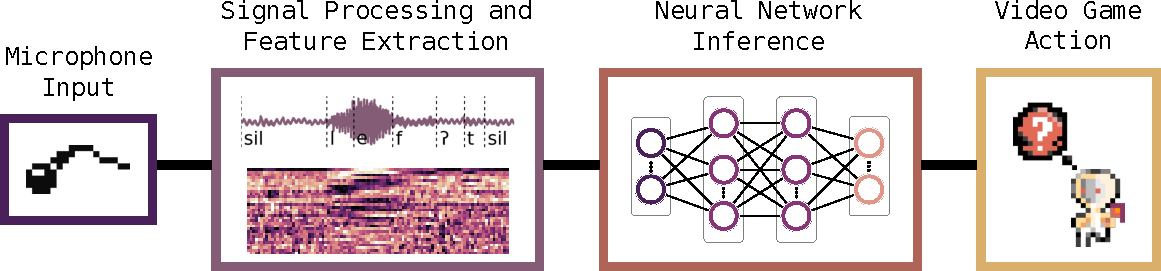
\includegraphics[width=1.0\textwidth]{../1_intro/figs/intro_kws.pdf} \end{figure}
\end{frame}

\begin{frame}
  \frametitle{KWS Problem Formulation}
  \begin{itemize}
    \item vocabulary with $L$ words:
    \begin{equation*}\label{eq:intro_kws_dict}
      S \coloneqq \{s_i \mid i = 0, 1, \dots, L - 1\},
    \end{equation*}

    \item closest word for target word $t$:
    \begin{equation*}\label{eq:intro_kws_task}
      \hat{s} = \underset{s_i \in S}{\arg \min} \, \mathcal{D}(t, s_i),
    \end{equation*}

    \item word prediction with neural network outputs $y_i$:
    \begin{equation*}\label{eq:intro_kws_class}
      \hat{s} = s_{\underset{i = 0, 1, \dots, L - 1}{\arg \max} \, y_i}
    \end{equation*}

  \end{itemize}
\end{frame}

% signal
% --
% intro

\section{Signal Processing and Feature Extraction}
\sectionheader{Signal Processing and Feature Extraction}
\begin{frame}
  \frametitle{*Speech Signals}
  \begin{itemize}
    \item Recorded with sample rate $f_s$
    \item Speech signal with $N$ samples:
    \begin{equation*}\label{eq:signal_raw_x}
      \bm{x} = [x_0, x_1, \dots, x_{N-1}]^T
    \end{equation*}
  \end{itemize}
  \begin{figure} 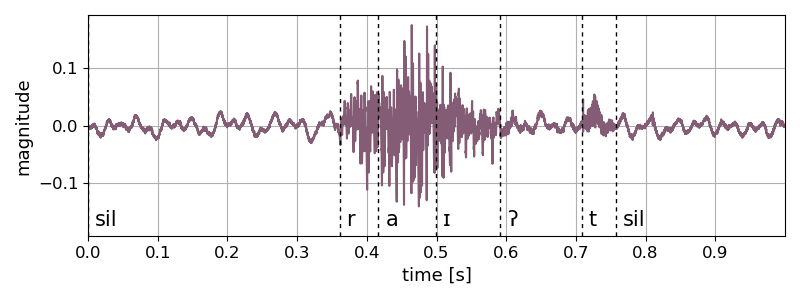
\includegraphics[width=0.65\textwidth]{../3_signal/figs/signal_raw_showcase_right0.png} \end{figure}
\end{frame}

\begin{frame}
  \frametitle{*Spectral Features}
  \begin{itemize}
    \item Discrete Fourier Transform (DFT):
    \begin{equation*}\label{eq:signal_spec_dtft_matrix}
      \footnotesize
      \begin{aligned}
        \hat{\bm{x}} = \mathcal{F} \bm{x} \quad & \mathrm{with} 
        \quad \mathcal{F}[k, n] = e^{-j\frac{2 \pi n}{N} k},\\
        &k, n = (0, 1, \dots, K-1), (0, 1, \dots, N-1)
      \end{aligned}
    \end{equation*}

    \item Short-Time Fourier Transform (STFT):
    \begin{equation*}\label{eq:signal_spec_stft}
      \footnotesize
      \begin{aligned}
        \tilde{X}[k, m] &= \sum_{n=0}^{N-1} x[n + m h] \, w[n] \, e^{-j\frac{2 \pi n}{N}k},\\ 
        m &= 0, 1, \dots, M - 1,\\
        M &= \ceil*{\frac{\norm{\bm{x}}_0-N}{h}}
      \end{aligned}
    \end{equation*}
  \end{itemize}
\end{frame}

\begin{frame}
  \frametitle{Spectral Features}
  \begin{columns}
    % lin
    \begin{column}{0.5\textwidth}
      \begin{itemize}
        \item linear Spectrogram:
        \begin{equation*}
          P = \abs{\tilde{X}}^2
        \end{equation*}
      \end{itemize}
      \begin{figure} 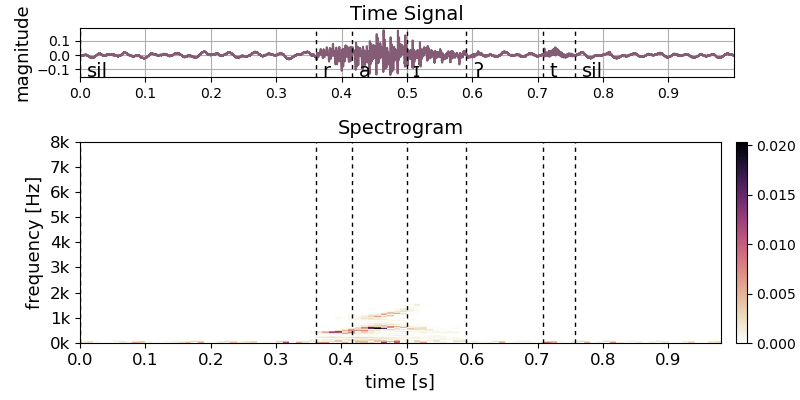
\includegraphics[width=1.0\textwidth]{../3_signal/figs/signal_spec-lin_showcase_right0.png} \end{figure}
    \end{column}
    % log
    \begin{column}{0.5\textwidth}
      \begin{itemize}
        \item logarithmic Spectrogram:
        \vspace{0.25cm}
        \begin{equation*}
          P_{DB} = 10 \cdot \log_{10}{P}
        \end{equation*}
      \end{itemize}
      \vspace{0.08cm}
      \begin{figure} 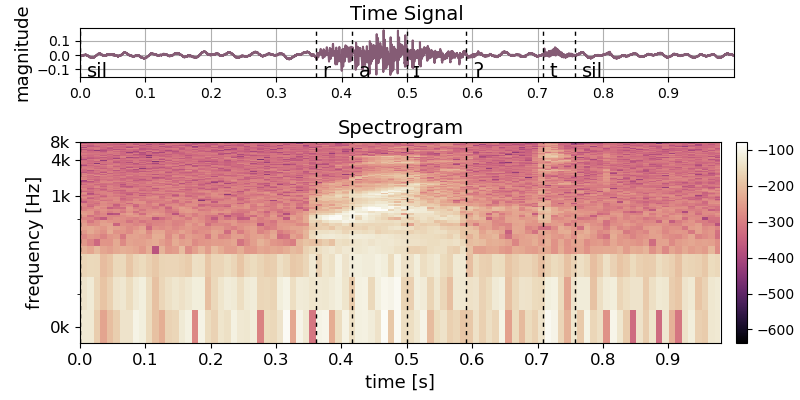
\includegraphics[width=1.0\textwidth]{../3_signal/figs/signal_spec-log_showcase_right0.png} \end{figure}
    \end{column}
  \end{columns}
\end{frame}

\begin{frame}
  \frametitle{*MFCC Features}
  \begin{itemize}
    \item Mel Frequency Cepstral Coefficient (MFCC):
    \begin{equation*}
      U = \mathcal{D} \log{ \left( W_m   P \right) }
    \end{equation*}
  \end{itemize}
  \begin{figure}
    \centering
    \subfloat[DCT ($\mathcal{D}$)]{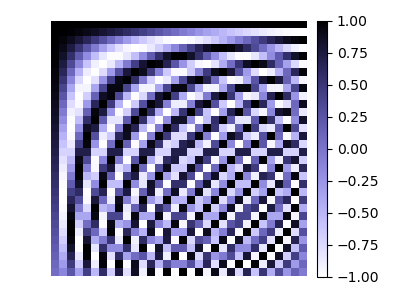
\includegraphics[width=0.45\textwidth]{../3_signal/figs/signal_mfcc_dct.png}}
    \subfloat[Mel Bands ($W_m$)]{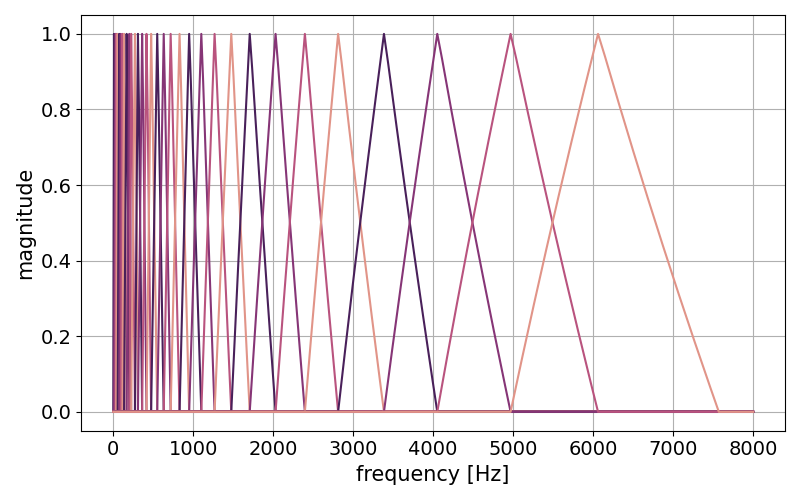
\includegraphics[width=0.5\textwidth]{../3_signal/figs/signal_mfcc_weights_f.png}}
  \end{figure}
\end{frame}

\begin{frame}
  \frametitle{MFCC Features}
  \begin{itemize}
    \item frame-based normalization:
    \vspace{0.2cm}
    \begin{equation*}
      \scriptsize
      \begin{aligned}
        &U[c, m] \gets \frac{U[c, m] + \vert \underset{m \in \mathcal{M}}{\min} \bm{u}_c \vert}{\norm{\bm{u}_c + \vert \underset{m \in \mathcal{M}}{\min} \bm{u}_c \vert}_\infty}\\
        & \forall \, c, m = (0, 1, \dots, C - 1), (0, 1, \dots, M - 1)
      \end{aligned}
    \end{equation*}
  \end{itemize}
  \vspace{-0.25cm}
  \begin{figure} 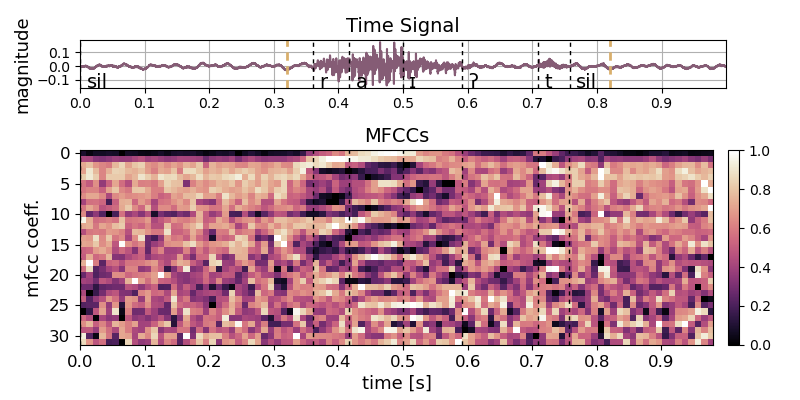
\includegraphics[width=0.65\textwidth]{../3_signal/figs/signal_mfcc_showcase_mfcc32_right0.png} \end{figure}
\end{frame}

\begin{frame}
  \frametitle{*MFCC Feature Enhancements}
  \begin{itemize}
    \item Delta- and Double Delta features:
    \vspace{0.2cm}
    \begin{equation*}
      \scriptsize
      \begin{aligned}
        \Delta u_c[m] = \frac{u_c[m - 1] + u_c[m + 1]}{2}
      \end{aligned}
    \end{equation*}
    \item Energy features:
    \begin{equation*}
      \scriptsize
      \begin{aligned}
        e[m] = \bm{u}[m]^T \bm{u}[m]
      \end{aligned}
    \end{equation*}
  \end{itemize}
  \begin{figure} 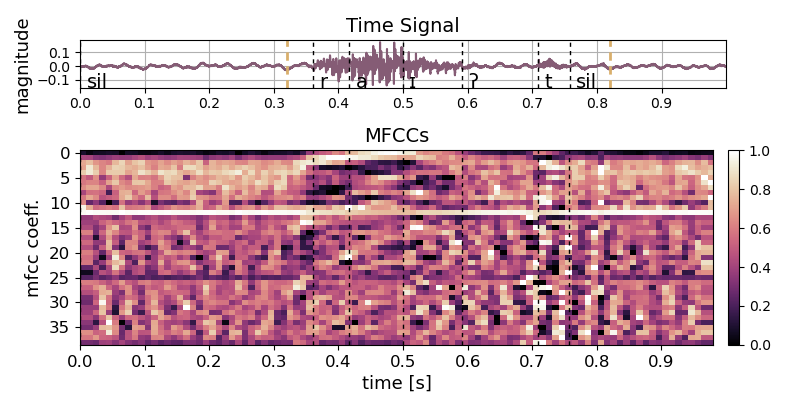
\includegraphics[width=0.65\textwidth]{../3_signal/figs/signal_mfcc_showcase_mfcc39_right0.png} \end{figure}
\end{frame}

\begin{frame}
  \frametitle{*MFCC Computations}
  \begin{itemize}
    \item signal: \SI{1}{\second} with $f_s = \SI{16}{\kilo\hertz}$.
    \item STFT and MFCC:
    \vspace{-0.1cm}
    \begin{itemize}
      \item \SI{25}{\milli\second} analytical window with \SI{10}{\milli\second} hop,
      \item $K = 400$ Fourier coefficients,
      \item $B = 32$ filter bands and 
      \item $C=12$ cepstral coefficients.
    \end{itemize}
  \end{itemize}
  \vspace{-0.5cm}
  \begin{table}[ht!]
\scriptsize
\begin{center}
\begin{tabular}{ M{5.5cm}  M{4cm} }
\toprule
\textbf{Process} & \textbf{Approximated Number of Operations} \\
\midrule
Power spectrum & \SI{2.71}{\mega\ops}\\
Weighting with equidistant Mel bands & \SI{1.26}{\mega\ops}\\
DCT transform of the weighted power spectrum & \SI{75}{\kilo\ops}\\
\midrule
\textbf{Sum} & \SI{4.05}{\mega\ops}\\
\bottomrule
\end{tabular}
\end{center}
\end{table}
\end{frame}

\begin{frame}
  \frametitle{Onset Detection}
  \begin{itemize}
    \item detect the start of keywords
    \item two kinds of onset detection method:
    \begin{itemize}
      \item keyword onset detection:
      \begin{itemize}
        \item find exact start of keyword in the audio file
        \item extraction of data examples with restricted time length (\SI{500}{\milli\second}).
      \end{itemize}
      \vspace{0.25cm}
      \item online onset detection:
      \begin{itemize}
        \item applied in the game to indicate whether a keyword is present.
      \end{itemize}
      \vspace{0.25cm}
      \begin{equation*}
        o(\bm{x}) = 
        \begin{cases}
          1, & \text{if } \frac{1}{n} \bm{x}^T \bm{x} > \alpha\\
          0, & \text{otherwise} 
        \end{cases},
      \end{equation*}
    \end{itemize}
  \end{itemize}
\end{frame}

\begin{frame}
  \frametitle{Keyword Onset Detection}
  \begin{columns}
    \begin{column}{0.5\textwidth}
      \begin{itemize}
        \item energy $e$ of each frame $m$:
        \begin{equation*}
          \footnotesize
          \begin{aligned}
            e[m] &= \sum_{i=0}^{N-1} \abs{x[m + i]}^2, \quad \mathrm{or}\\
            e[m] &= \sum_{i=0}^{N-1} u_0[m + i],\\
          \end{aligned}
        \end{equation*}

         \item onset $o$:
        \begin{equation*}
          \footnotesize
          \begin{aligned}
            o &= \underset{m \in \mathcal{M}}{\arg \max} \, e[m]
          \end{aligned}
        \end{equation*}
      \end{itemize}
    \end{column}
    \begin{column}{0.5\textwidth}
      \centering
      \begin{figure} \hspace{0.75cm} 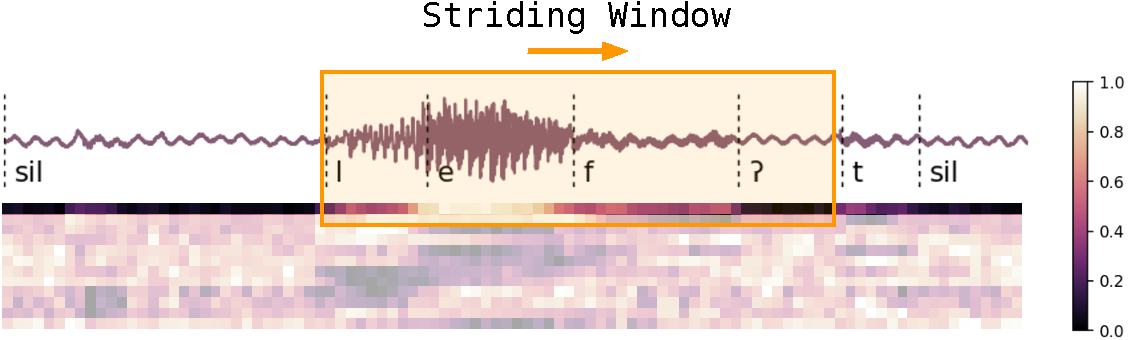
\includegraphics[width=1.0\textwidth]{../3_signal/figs/signal_onset_window.pdf} \end{figure}
      \begin{figure} 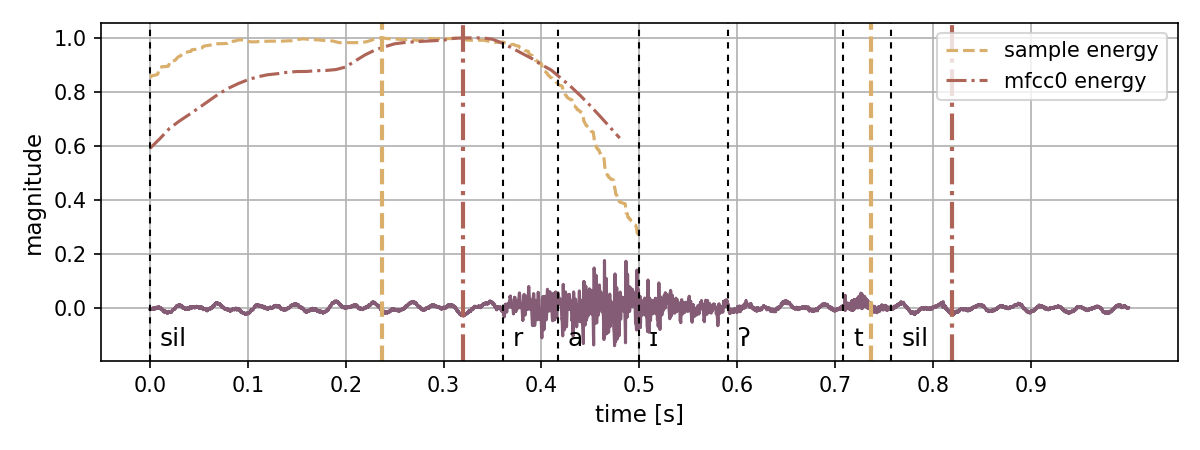
\includegraphics[width=1.0\textwidth]{../3_signal/figs/signal_onset_showcase_right0.png} \end{figure}
      \vfill
    \end{column}
  \end{columns}
\end{frame}

% ml
% --
% machine learning

\section{Neural Networks for KWS}
\sectionheader{Neural Networks for KWS}

\begin{frame}
  \frametitle{Neural Network approaches}
  \begin{itemize}
    \item Convolutional Neural Networks (CNNs)
    \begin{itemize}
      \item MFCCs as input features
      \item simple network architectures with different striding properties adapted from \cite{Sainath2015KWS}
    \end{itemize}
    \item Generative Adversarial Neural Networks (GANs) \cite{Goodfellow2014GANs}
    \begin{itemize}
      \item used to improve the classification performance of equivalent CNN models
    \end{itemize}
    \item Wavenets \cite{Oord2016Wavenet}
    \begin{itemize}
      \item raw audio data as input features
      \item no feature extraction
    \end{itemize}
  \end{itemize}
\end{frame}

\begin{frame}
  \frametitle{*Fully Connected Layer}
  \begin{columns}
    \begin{column}{0.45\textwidth}
      \begin{itemize}
        \item output $z$ with activation $h$:
        \begin{equation*}
          \footnotesize
          \begin{aligned}
            \bm{z} = h(W \bm{x} + \bm{b})
          \end{aligned}
        \end{equation*}
        {\scriptsize with $\bm{x} \in \R^n$, $\bm{z} \in \R^m$, $\bm{b} \in \R^m$.}
        \vspace{0.2cm}
        \item amount of parameters:
        \begin{equation*}
          \footnotesize
          \begin{aligned}
            m \cdot n + m
          \end{aligned}
        \end{equation*}
        \item amount of operations:
        \begin{equation*}
          \footnotesize
          \begin{aligned}
            \mathcal{T}(W \bm{x} + \bm{b}) \approx 2 (m \cdot n) + m
          \end{aligned}
        \end{equation*}
      \end{itemize}
    \end{column}
    \begin{column}{0.55\textwidth}
      \vspace{0.75cm}
      \centering
      \begin{figure} 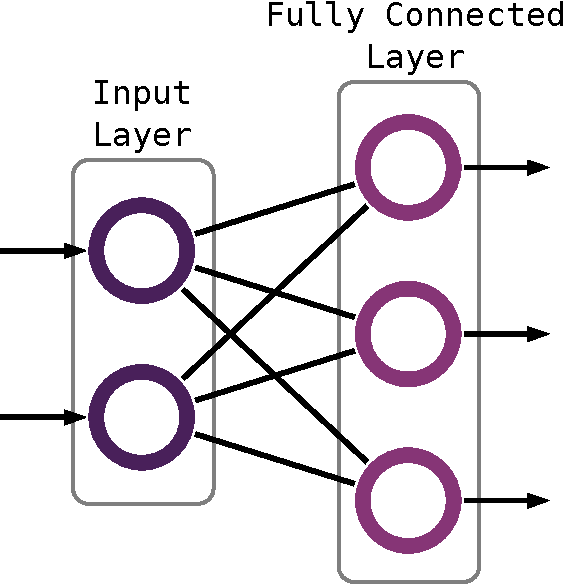
\includegraphics[width=0.55\textwidth]{../4_nn/figs/nn_theory_fc.pdf} \end{figure}
      \vfill
    \end{column}
  \end{columns}
\end{frame}

\begin{frame}
  \frametitle{*Convolutional Layer}
  \vspace{-0.5cm}
  \begin{columns}
    \begin{column}{0.6\textwidth}
      \begin{itemize}
        \item output dimension through kernel stride:
        \begin{equation*}\label{eq:nn_theory_cnn_dim}
        d_{o_z} = \floor*{\frac{d_{x_z} + p_z - d_{k_z}}{s_z} + 1},
        \end{equation*}
        {\footnotesize
        with $z$: dimensional axis, $d_{x}$: input dim, $p$: padding, $k$: kernel size, $s$: stride}.
        \item j-th output channel $o_j$:
        \begin{equation*}
          \footnotesize
          o_j = \sum_{i} k_{i, j} \ast x_i,
        \end{equation*}
        \footnotesize
        with $x_i$ as i-th input channel and $k_{i, j}$ as kernel.   
      \end{itemize}
    \end{column}
    \begin{column}{0.4\textwidth}
      \vspace{1cm}
      \begin{figure} 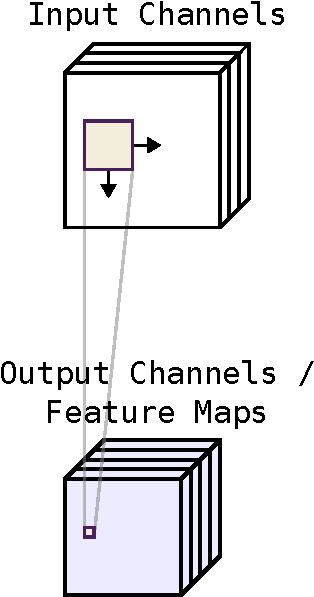
\includegraphics[width=0.5\textwidth]{./figs/nn_theory_cnn_scheme.pdf} \end{figure}
    \end{column}
  \end{columns}
\end{frame}

\begin{frame}
  \frametitle{Convolutional Layer Example}
  \vspace{0.2cm}
  \begin{figure} 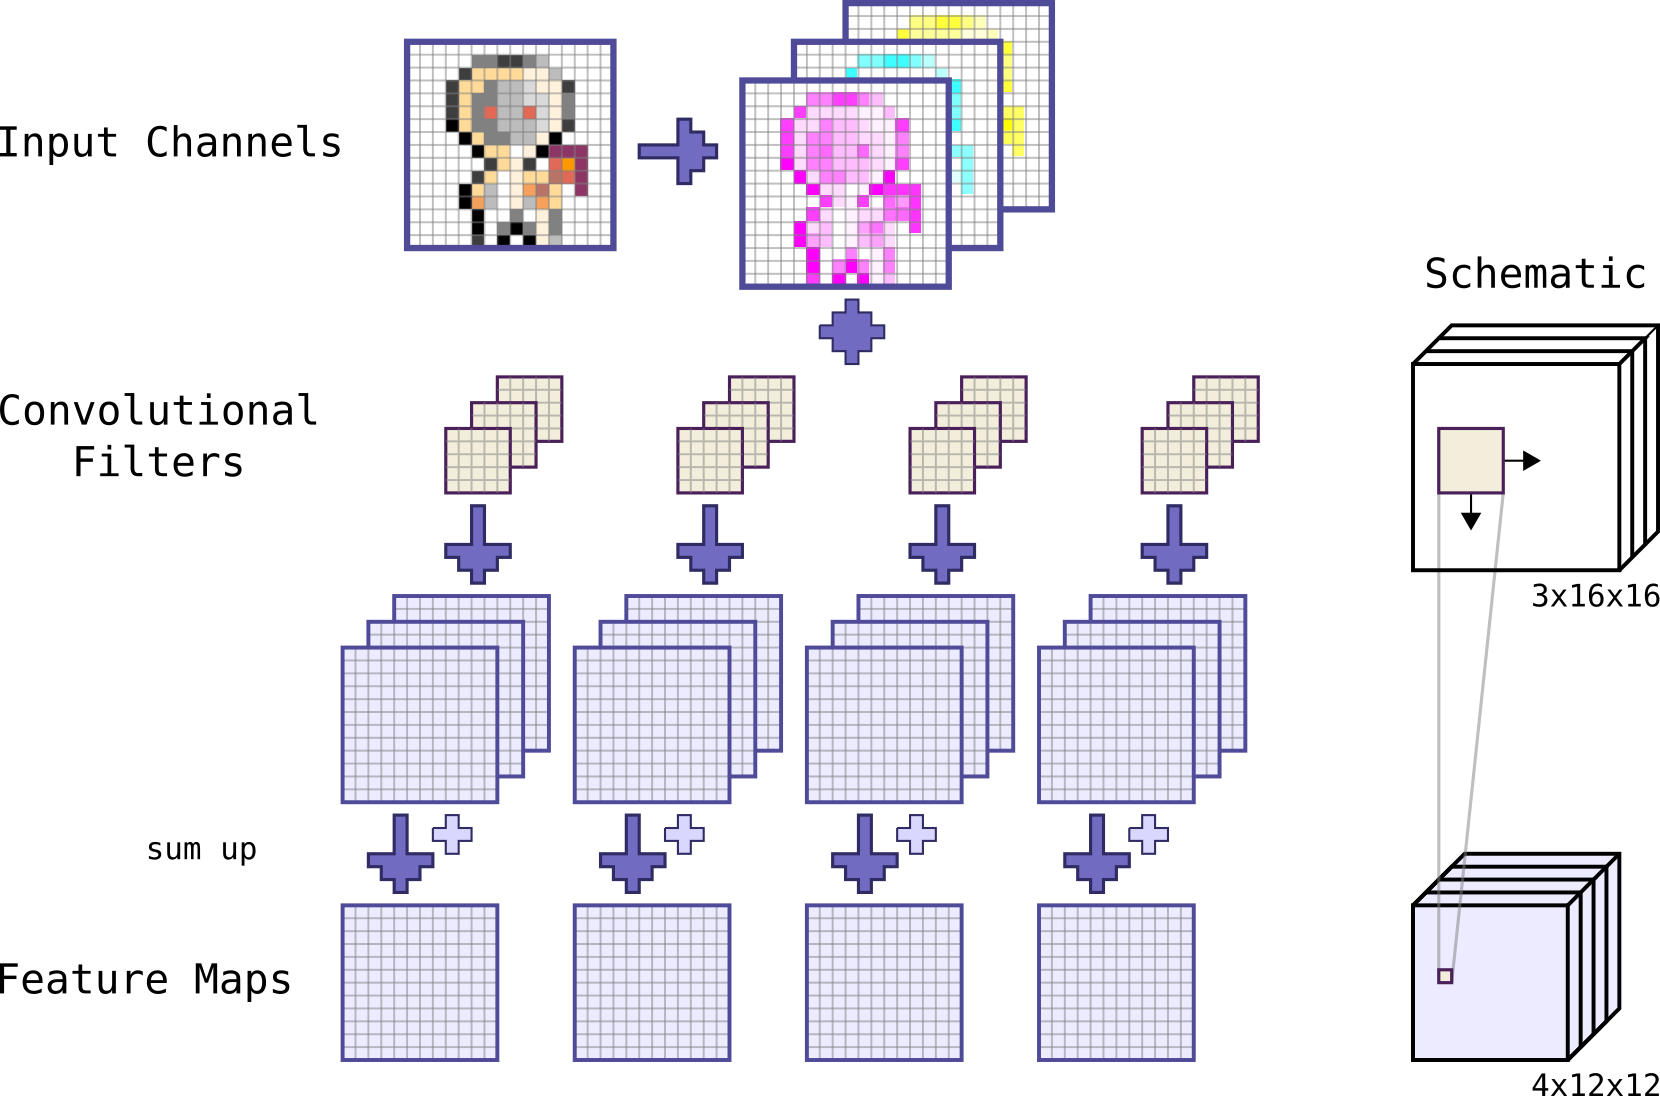
\includegraphics[width=0.8\textwidth]{./figs/nn_theory_cnn_basics.png} \end{figure}
\end{frame}

\begin{frame}
  \frametitle{Striding properties of CNNs}
  \begin{itemize}
    \item striding of the conv. filters (kernels) from the first conv. layers of all three CNN models:
  \end{itemize}
  \hspace{1cm}
  \scalebox{0.75}
  {
    \begin{tikzpicture}
      \node at (0, 0) (ktrad) [inner sep=0] {
\includegraphics[width=0.5\textwidth]{./figs/real_right_sample.png}};
      \node [below=of ktrad, inner sep=0] (kfstride) {
\includegraphics[width=0.5\textwidth]{./figs/real_right_sample.png}};
      \node [below=of kfstride, inner sep=0] (kjim) {
\includegraphics[width=0.5\textwidth]{./figs/real_right_sample.png}};

      % fstride
      \draw [color=neonlightblue, line width=1.5pt] (ktrad.north west) rectangle ++(62pt, -0.45cm);
      \draw [->, line width=1.0pt, color=neonlightblue] ($(ktrad.west) + (65pt, 13pt)$) -- ++(8pt, 0);
      \draw [->, line width=1.0pt, color=neonlightblue] ($(ktrad.south) + (-48pt, 0.8cm)$) -- ++(0, -8pt);

      % fstride
      \draw [color=neonlightblue, line width=1.5pt] (kfstride.north west) rectangle ($(kfstride.north east) + (0, -0.9cm)$);
      \draw [->, line width=1.0pt, color=neonlightblue] ($(kfstride.south) + (0, 0.35cm)$) -- ++(0, -8pt);

      % fstride
      \draw [color=neonlightblue, line width=1.5pt] (kjim.north west) rectangle ($(kjim.south west) + (62pt, 0)$);
      \draw [->, line width=1.0pt, color=neonlightblue] ($(kjim.west) + (65pt, 0)$) -- ++(8pt, 0);

      % text
      \node at (ktrad.west) [xshift=-2pt, anchor=east] {\texttt{conv-trad}};
      \node at (kfstride.west) [xshift=-2pt, anchor=east] {\texttt{conv-fstride}};
      \node at (kjim.west) [xshift=-2pt, anchor=east] {\texttt{conv-jim}};
    \end{tikzpicture}
  }
\end{frame}

\begin{frame}
  \frametitle{Traditional Network (\texttt{conv-trad})}
  \begin{itemize}
    \item layer structure: conv.: 2 + 1 max. pool, FC: 3
    \item num. parameters: \textbf{\num{68396}}
    \item num. operations: \textbf{\SI{3770.98}{\kilo\ops}}
  \end{itemize}
  \begin{figure} 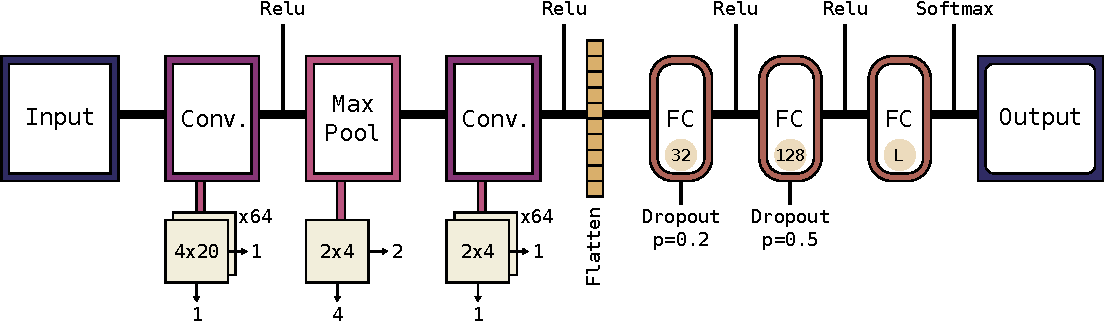
\includegraphics[height=0.35\textheight]{../4_nn/figs/nn_arch_cnn_trad.pdf} \end{figure}
\end{frame}

\begin{frame}
  \frametitle{Frequency Striding Network (\texttt{conv-fstride})}
  \begin{itemize}
    \item layer structure: conv.: 1, FC: 4
    \item num. parameters: \textbf{\num{47426}} 
    \item num. operations: \textbf{\SI{137.75}{\kilo\ops}}
  \end{itemize}
  \begin{figure} 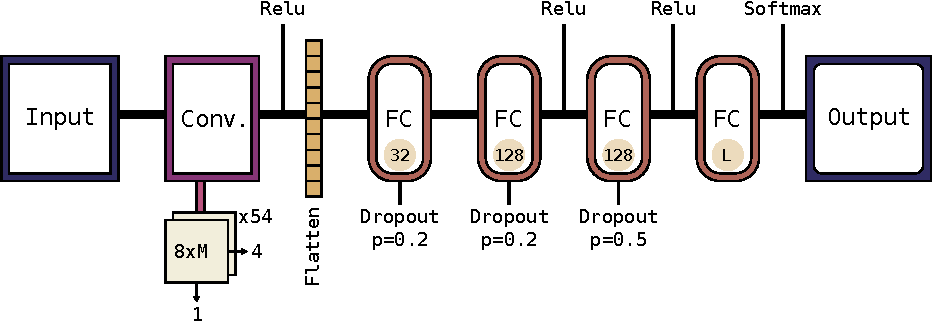
\includegraphics[height=0.35\textheight]{../4_nn/figs/nn_arch_cnn_fstride.pdf} \end{figure}
\end{frame}

\begin{frame}
  \frametitle{Time Striding Network (\texttt{conv-jim})}
  \begin{itemize}
    \item layer structure: conv.: 2, FC: 3
    \item num. parameters: \textbf{\num{29804}}
    \item num. operations: \textbf{\SI{862.40}{\kilo\ops}}
  \end{itemize}
  \begin{figure} 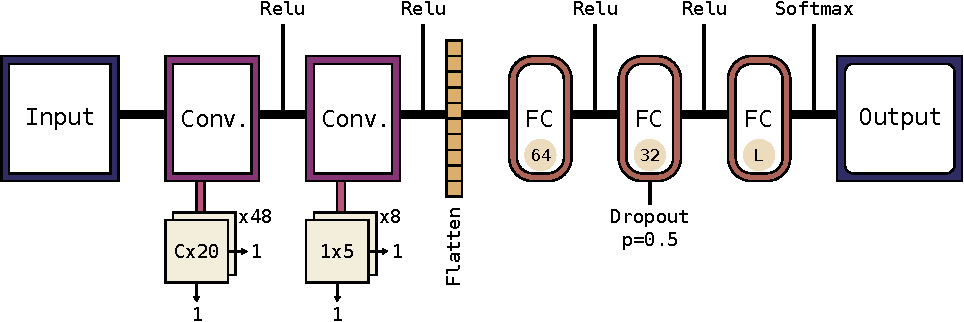
\includegraphics[height=0.35\textheight]{../4_nn/figs/nn_arch_cnn_jim.pdf} \end{figure}
\end{frame}

\begin{frame}
  \frametitle{GANs}
  \begin{itemize}
    \item consist of two adversarial networks:
    \begin{itemize}
      \footnotesize
      \item Discriminator (D): classify images to fake or real  $D: \mathcal{X} \mapsto [0, 1]$ .
      \item Generator (G): produce new data examples $G: \mathcal{Z} \mapsto \mathcal{X}$.
    \end{itemize}
    \begin{tikzpicture} 
      \node at (0, 0) (g) {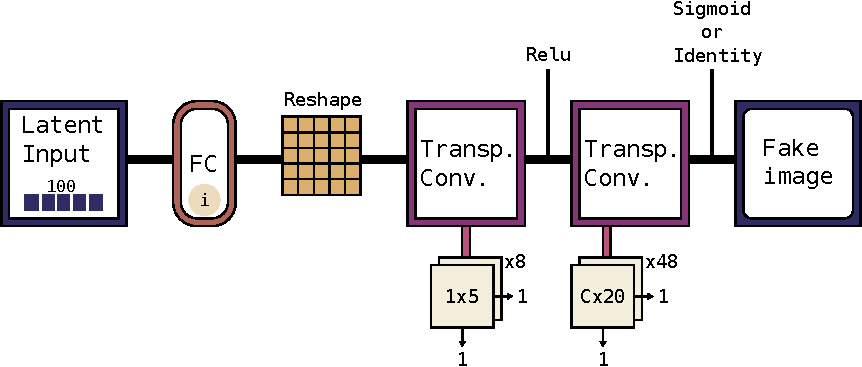
\includegraphics[width=0.4\textwidth]{../4_nn/figs/nn_arch_adv_g_jim.pdf}};
      \node at (g.east)[yshift=0.1cm] (vs) [anchor=west, font=\bf] {vs.};
      \node at (vs.east)[yshift=-0.2cm] (d) [anchor=west] {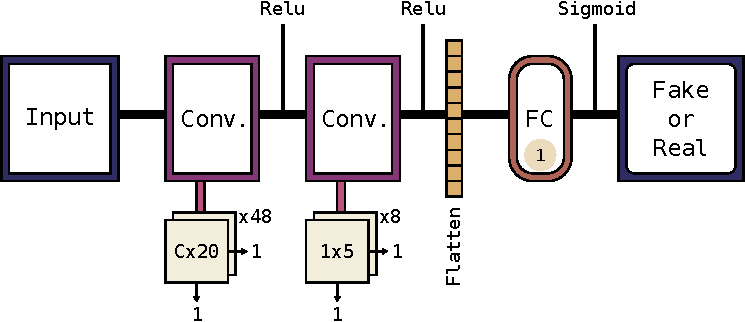
\includegraphics[width=0.35\textwidth]{../4_nn/figs/nn_arch_adv_d_jim.pdf}};
      \node at (vs.south)[yshift=-0.3cm] (sample) [anchor=north, rectangle, draw=blue!25!black, inner sep=2pt, line width=1pt] {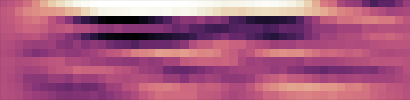
\includegraphics[width=0.10\textwidth]{./figs/nn_adv_generated_sample.png}};
      % lines
      \draw [<-] [color=blue!25!black, line width=0.5pt] (sample.west) -- ++(-0.20cm, 0cm) -- ++(0, 0.4cm);
      \draw [->] [color=blue!25!black, line width=0.5pt] (sample.east) -- ++(0.20cm, 0cm) -- ++(0, 0.4cm);
      % text above
      \node at (g.north west) [xshift=0.6cm, yshift=-0.1cm, anchor=north east] {\scriptsize G};
      \node at (d.north west) [xshift=0.6cm, yshift=0.1cm, anchor=north east] {\scriptsize D};
    \end{tikzpicture}
    \vspace{0.2cm}
    \item Min-Max solution for the game between G and D:
  \end{itemize}
  \begin{equation*}
    \footnotesize
    \begin{aligned}
      \underset{G}{\min} \, \underset{D}{\max} \, V(D, G) = \quad & \E_{\bm{x} \sim p_{data}(\bm{x})}\left[ \log D(\bm{x}) \right] + \\
      & \E_{\bm{z} \sim p_{\bm{z}}(\bm{z})}\left[ \log (1 - D(G(\bm{z}))) \right],
    \end{aligned}
  \end{equation*}
\end{frame}

\begin{frame}
  \frametitle{*GAN training losses}
  \begin{itemize}
    \item binary cross entropy loss $l$:
    \begin{equation*}
      \footnotesize
      \begin{aligned}
        l(x_i, y_i) = y_i \cdot \log x_i + (1 - y_i) \cdot \log (1 - x_i)
      \end{aligned}
    \end{equation*}
    \item loss of D ($y_r$: real-, $y_f$: fake-label):
    \begin{equation*}
      \footnotesize
      \begin{aligned}
        l_D(x_i, z_i, G) = l(D(x_i), y_r) + l(D(G(z_i)), y_f)
      \end{aligned}
    \end{equation*}
    \item loss of G:
    \begin{equation*}
      \footnotesize
      \begin{aligned}
        l_G(z_i, D) =  l(D(G(z_i)), y_r)
      \end{aligned}
    \end{equation*}
    \item loss of G with similarity term ($s$ is cosine similarity):
    \begin{equation*}
      \footnotesize
      \begin{aligned}
        l_G(x_i, z_i, D) =  l(D(G(z_i)), y_r) + \lambda \left(1 - \frac{1}{C} \sum_{c=0}^{C} s(\hat{\bm{e}}_c^T x_i , \hat{\bm{e}}_c^T G(z_i)) \right),
      \end{aligned}
    \end{equation*}
  \end{itemize}
\end{frame}

\begin{frame}
  \frametitle{Adversarial Label Training}
  \begin{itemize}
    \item individual training instances on label subsets:
  \end{itemize}
  \begin{figure} 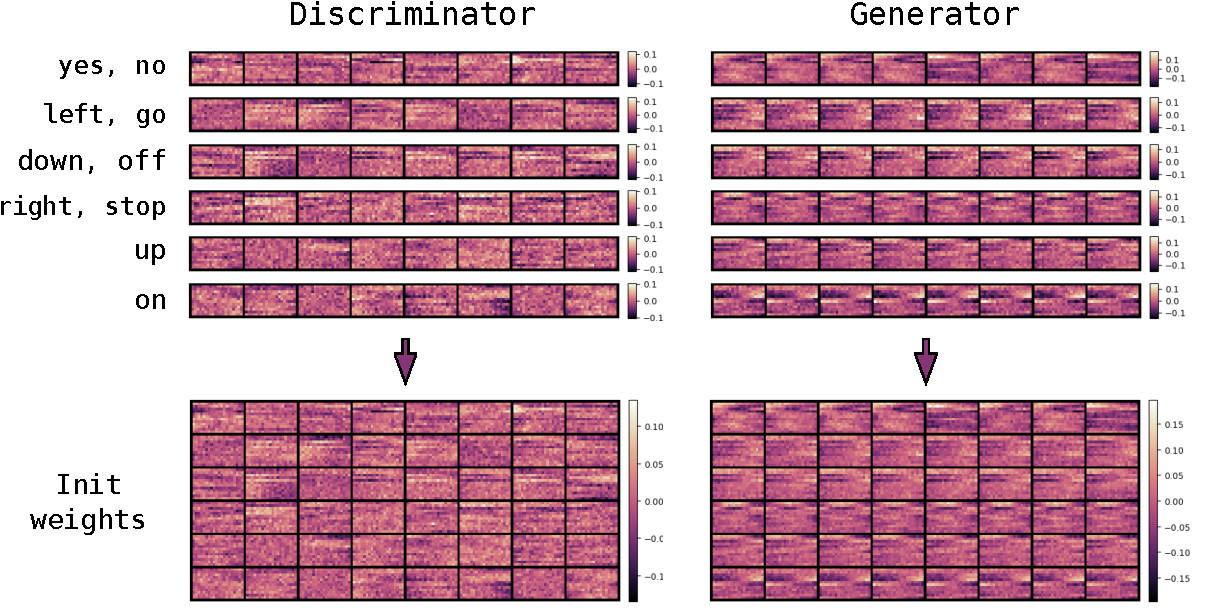
\includegraphics[height=0.7\textheight]{../4_nn/figs/nn_adv_label_scheme.pdf} \end{figure}
\end{frame}

\begin{frame}
  \frametitle{Adversarial Label Training}
  \begin{itemize}
    \item training on label \enquote{right} without similarity term:
  \end{itemize}
    \begin{tikzpicture} 
      \node at (0, 0) (a) {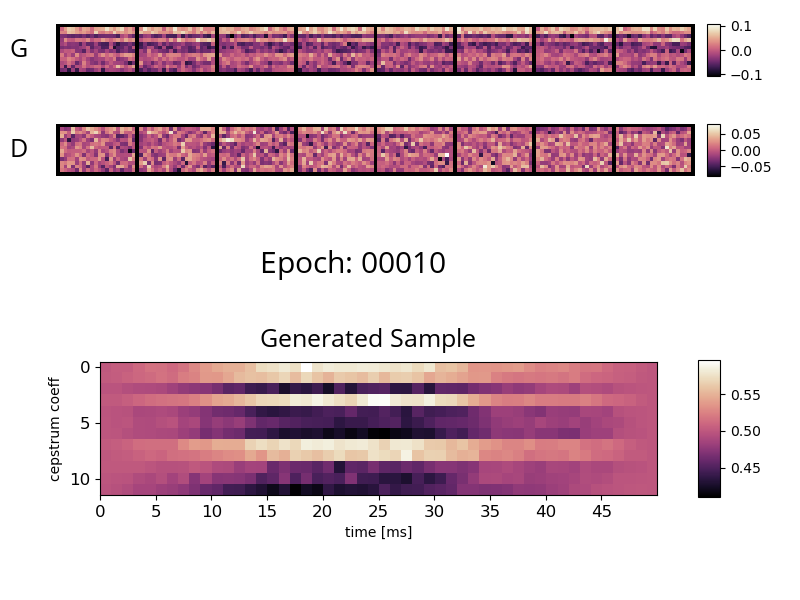
\includegraphics[width=0.4\textwidth]{./figs/adv_experimental_ep-10}};
      \node at (a.east)[xshift=0.2cm] (b) [anchor=west] {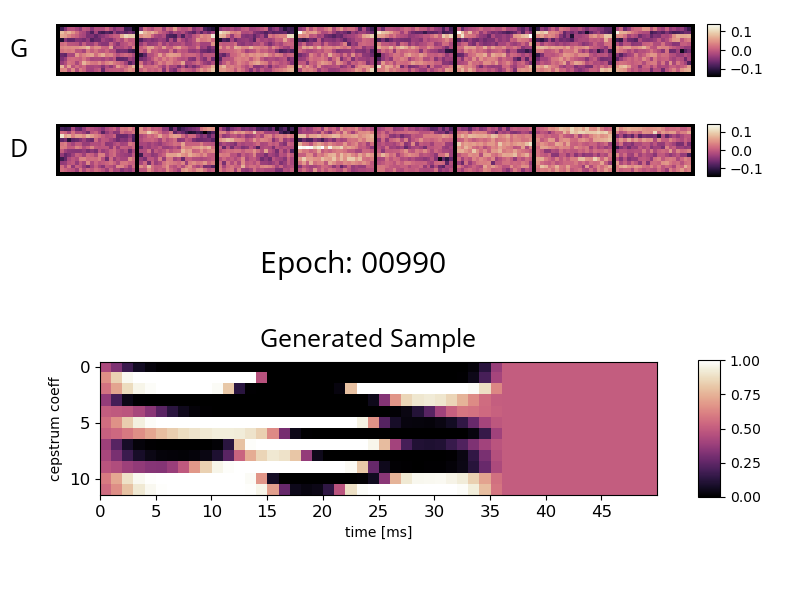
\includegraphics[width=0.4\textwidth]{./figs/adv_experimental_ep-990}};
      \node at (a.south) (c) [anchor=north] {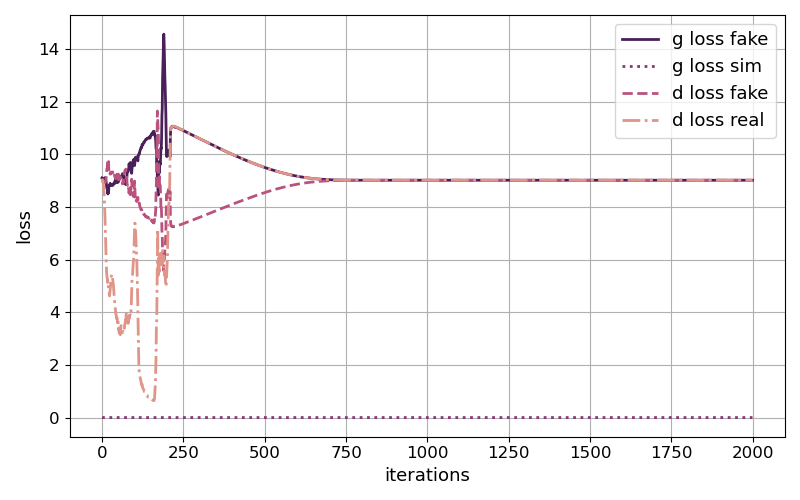
\includegraphics[width=0.4\textwidth]{./figs/adv_experimental_loss}};
      % lines
      \draw [->] [color=blue!25!black, line width=1.5pt] (a.east) -- ++(6pt, 0cm);
    \end{tikzpicture}
\end{frame}

\begin{frame}
  \frametitle{Adversarial Label Training}
  \begin{itemize}
    \item training on label \enquote{right} with similarity term:
  \end{itemize}
    \begin{tikzpicture} 
      \node at (0, 0) (a) {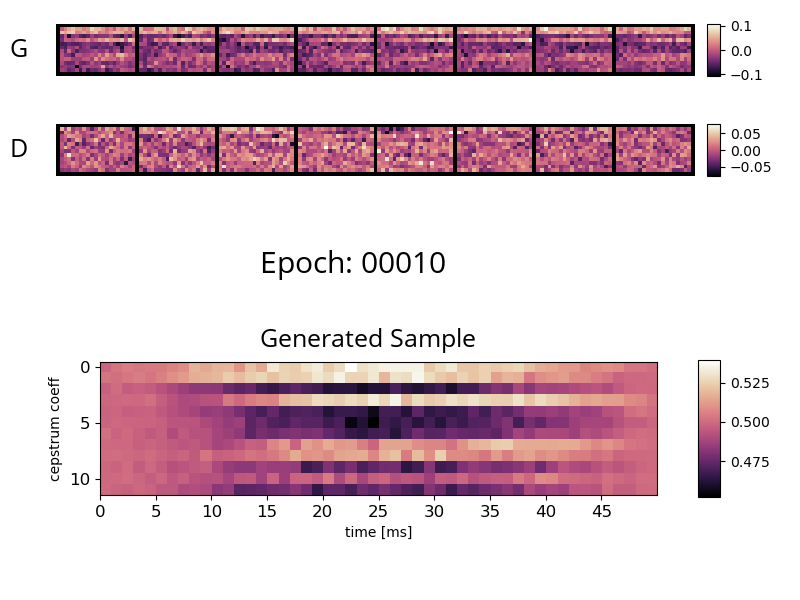
\includegraphics[width=0.4\textwidth]{./figs/adv_conv-jim_ep-10}};
      \node at (a.east)[xshift=0.2cm] (b) [anchor=west] {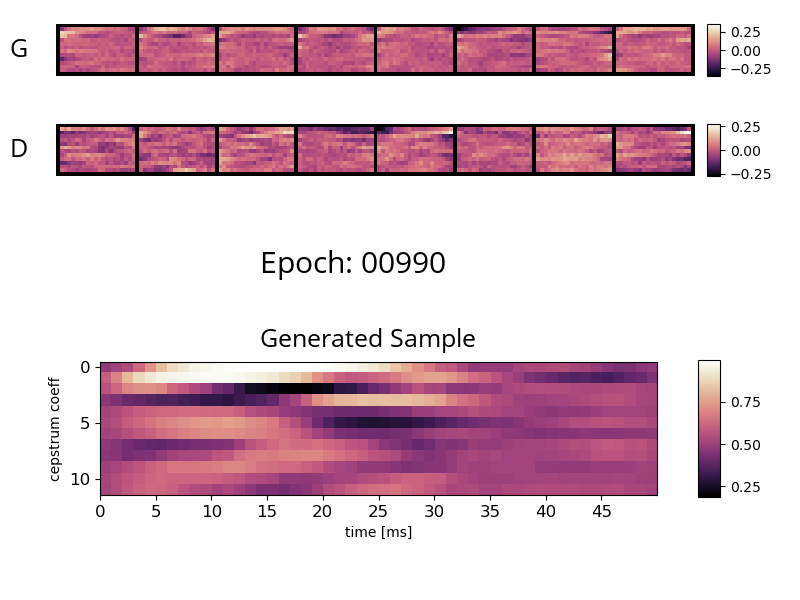
\includegraphics[width=0.4\textwidth]{./figs/adv_conv-jim_ep-990}};
      \node at (a.south) (c) [anchor=north] {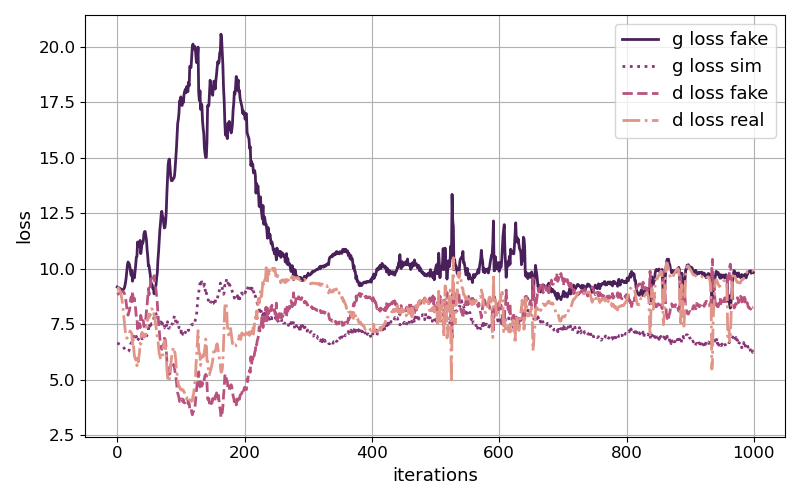
\includegraphics[width=0.4\textwidth]{./figs/adv_conv-jim_loss}};
      % lines
      \draw [->] [color=blue!25!black, line width=1.5pt] (a.east) -- ++(6pt, 0cm);
    \end{tikzpicture}
\end{frame}

\begin{frame}
  \frametitle{*Wavenets}
  \begin{itemize}
    \item perform  on raw audio data ($\SI{1}{\second}$ = 16000 features)
    \item key techniques: 
    \begin{itemize}
      \item dilated convolutions
      \item quantization of audio samples (256 values)
    \end{itemize}
    \item residual block schematic:
  \end{itemize}
  \vspace{-0.2cm}
  \begin{figure} 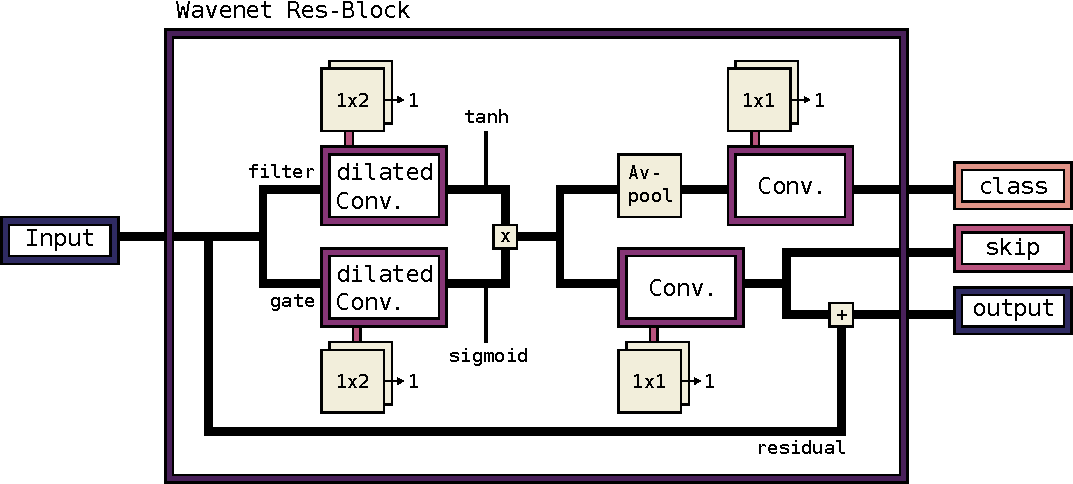
\includegraphics[height=0.35\textheight]{../4_nn/figs/nn_arch_wavenet_block.pdf} \end{figure}
\end{frame}

\begin{frame}
  \frametitle{Wavenet Architecture}
  \begin{itemize}
    \item num. parameters: \textbf{\num{33509}}
    \item num. operations: \textbf{\SI{36695.02}{\kilo\ops}}
  \end{itemize}
  \vspace{-0.2cm}
  \begin{figure} 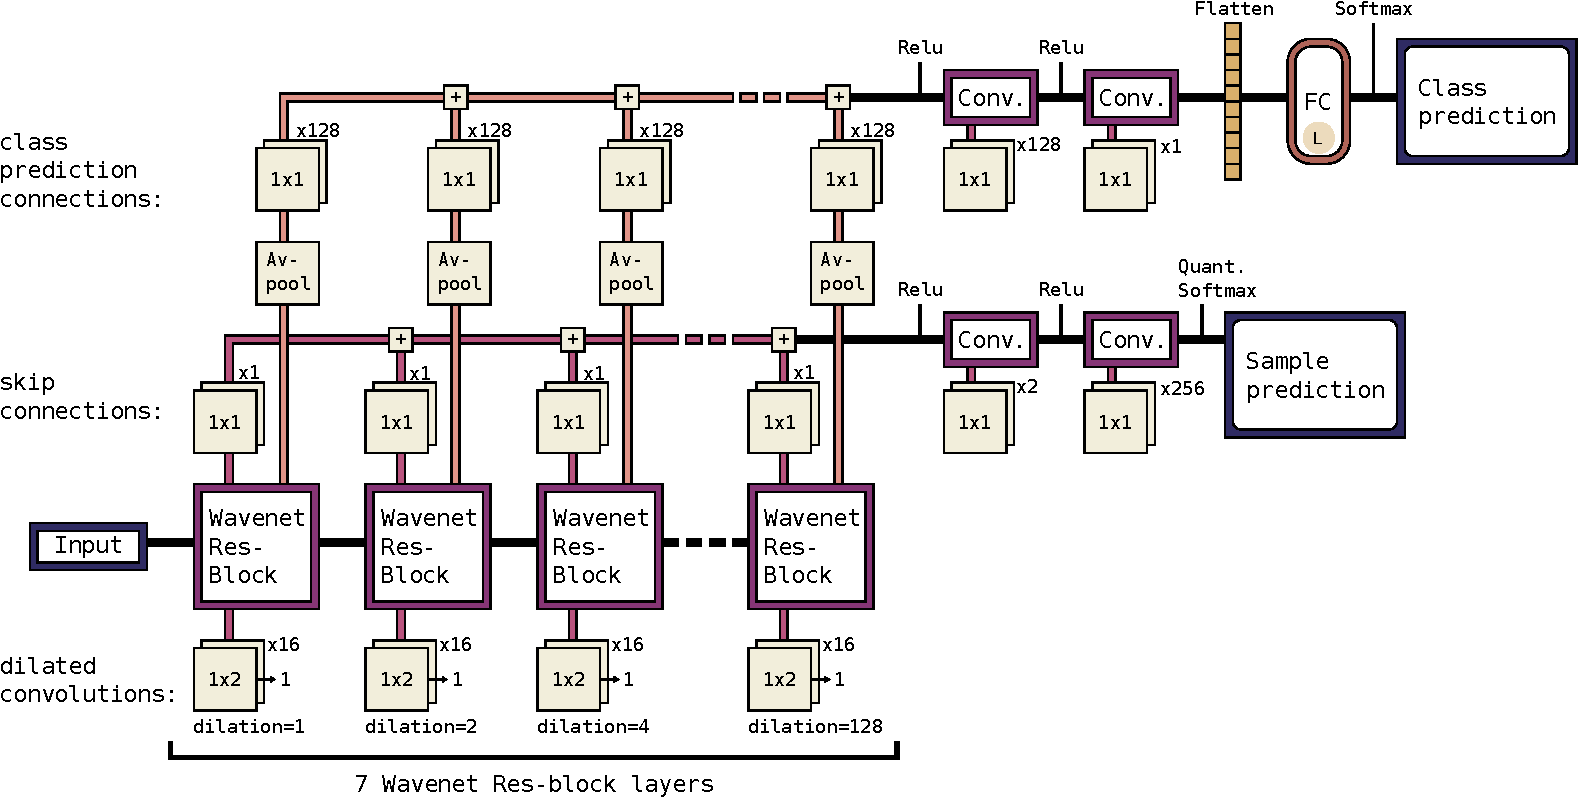
\includegraphics[height=0.6\textheight]{../4_nn/figs/nn_arch_wavenet_all.pdf} \end{figure}
\end{frame}

% experiments
% --
% experiments

\section{Experiments}
\sectionheader{Experiments}

\begin{frame}
  \frametitle{Speech Commands Dataset \texttt{v0.02}.}
  \begin{itemize}
    \item contains a large range of different quality recordings
    \item labels can be split into core- and auxiliary-keywords
  \end{itemize}
  \vspace{-0.5cm}
  \begin{columns}
    \begin{column}{0.55\textwidth}
    \centering
    \begin{table}[ht!]
\scriptsize
\begin{center}
\begin{tabular}{ M{3cm}  M{1.5cm} }
\toprule
Total number of keywords & 35\\
Number of core keywords & 20\\
Number of auxiliary keywords & 15\\
\midrule
Total number of examples & 105886\\
Total number of speakers & 2618\\
\midrule
Recording duration & 0.4 - \SI{1}{\second}\\
Channels & Mono\\
Bit depth of audio files & \SI{32}{\bit}\\
Sampling frequency & \SI{16}{\kilo\hertz}\\
\bottomrule
\label{tab:exp_dataset_hard_facts}
\end{tabular}
\end{center}
\end{table}


    \end{column}
    \begin{column}{0.45\textwidth}
      \centering
      \begin{figure} 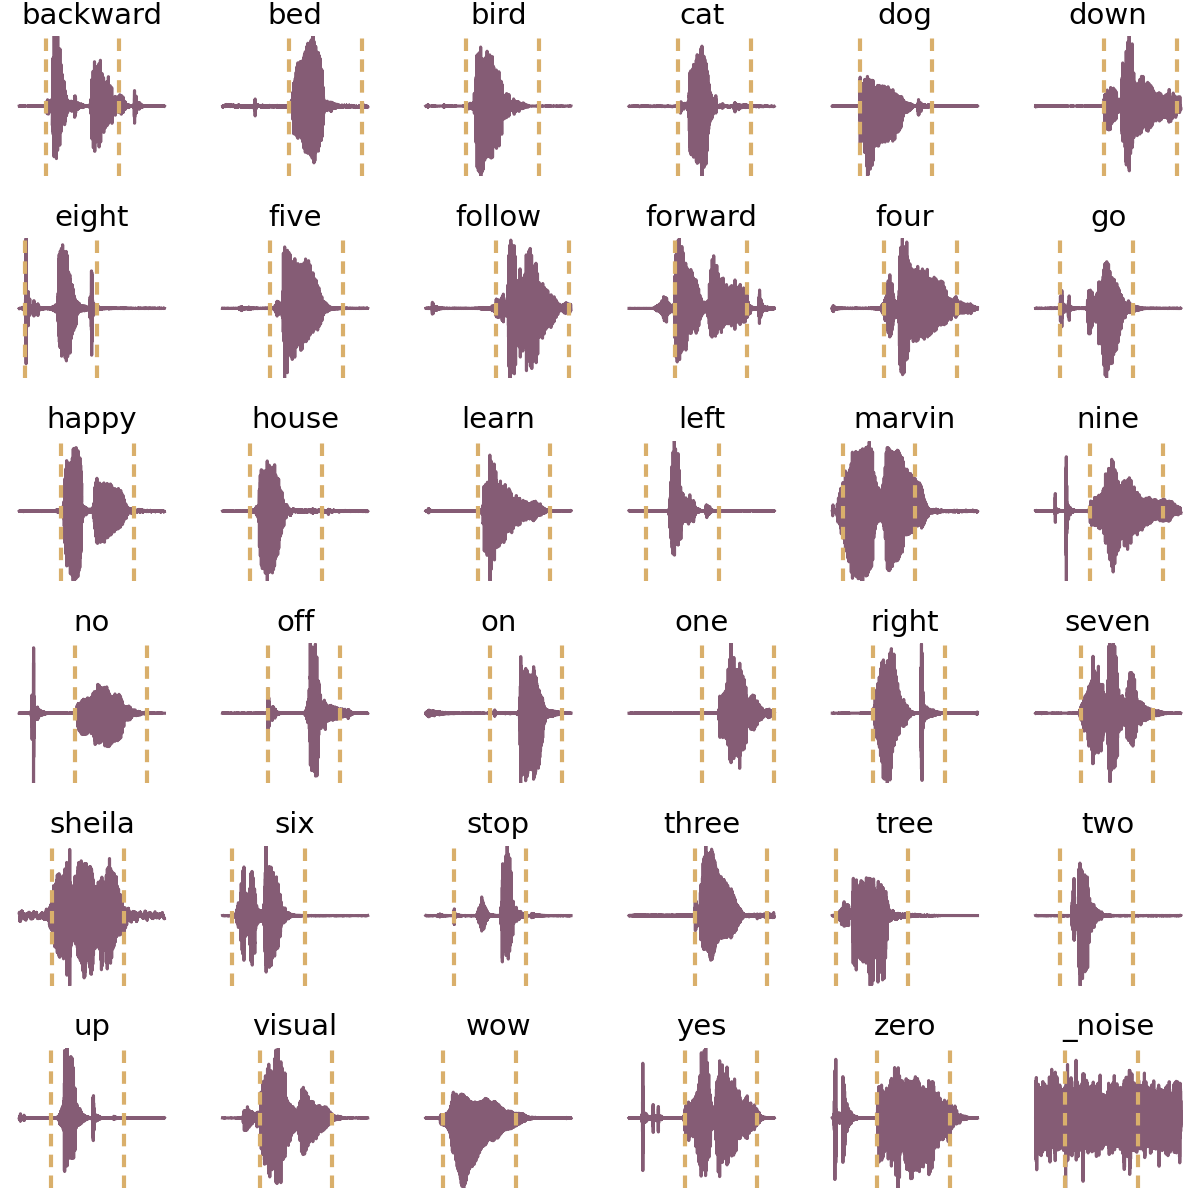
\includegraphics[width=0.9\textwidth]{../5_exp/figs/exp_dataset_speech_cmd_wav_grid.png} \end{figure}
    \end{column}
  \end{columns}
\end{frame}

\begin{frame}
  \frametitle{MFCC Extracted Dataset Examples}
  \vspace{-0.5cm}
  \begin{figure}[!ht]
    \centering
    \subfloat[left]{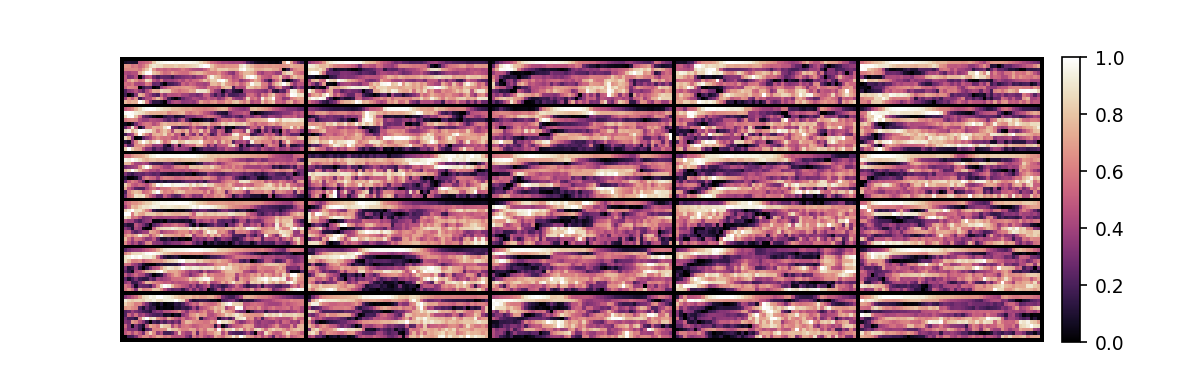
\includegraphics[width=0.8\textwidth]{../5_exp/figs/exp_dataset_speech_cmd_mfcc_left.png}}\\
    \vspace{-0.1cm}
    \subfloat[right]{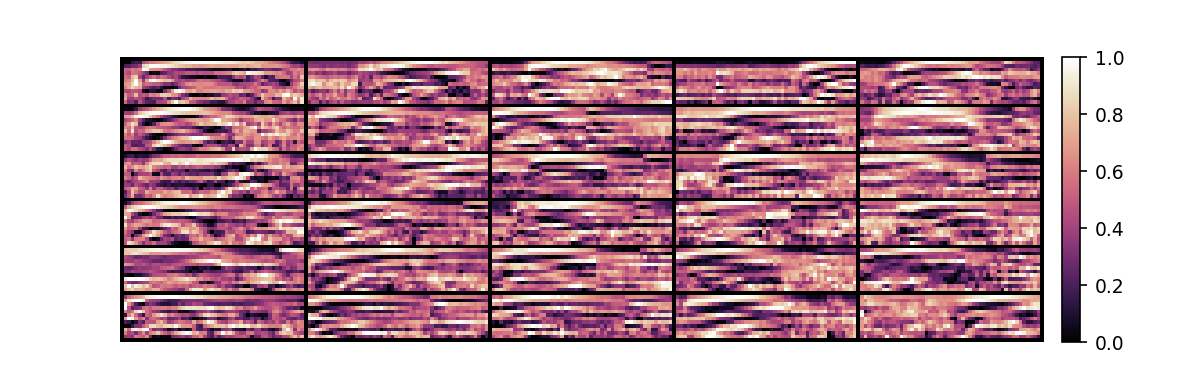
\includegraphics[width=0.8\textwidth]{../5_exp/figs/exp_dataset_speech_cmd_mfcc_right.png}}
  \end{figure}
\end{frame}

\begin{frame}
  \frametitle{My Dataset}
  \begin{itemize}
    \item vocabulary: \{\enquote{left}, \enquote{right}, \enquote{up}, \enquote{down}, \enquote{go}\}
    \item 5 examples per label
    \item used as additional test set
  \end{itemize}
  \vspace{-0.3cm}
  \begin{figure}[!ht]
    \centering
    \subfloat[audio]{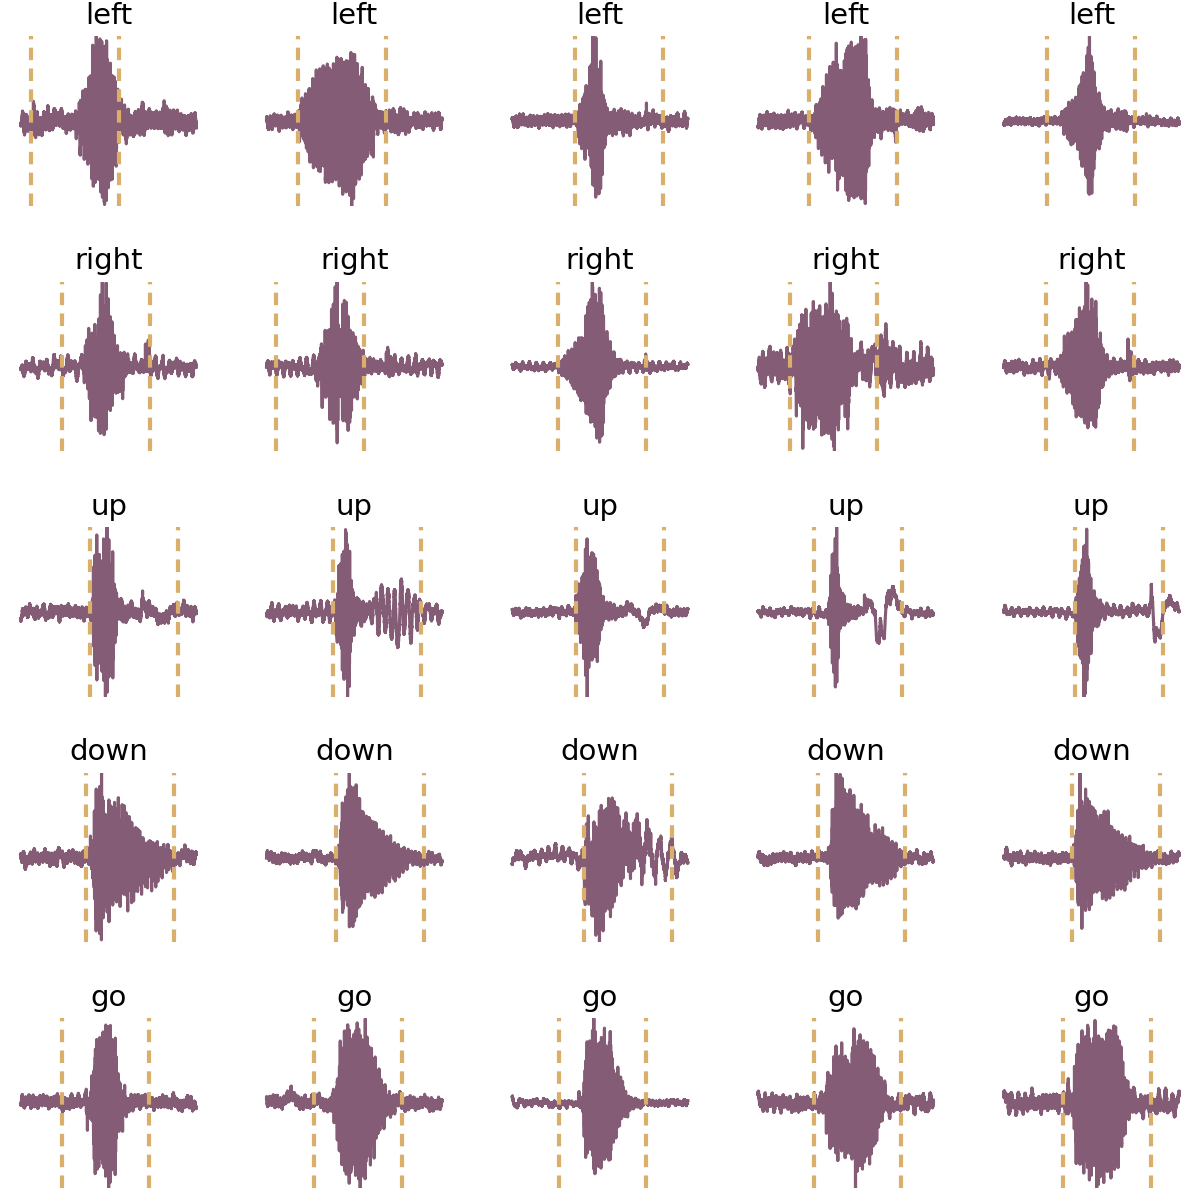
\includegraphics[width=0.29\textwidth]{../5_exp/figs/exp_dataset_my_wav_grid.png}}
    \subfloat[MFCC]{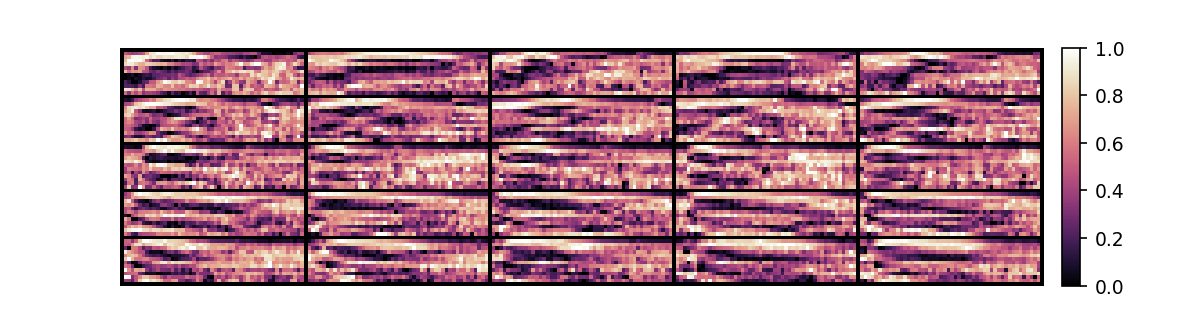
\includegraphics[width=0.69\textwidth]{../5_exp/figs/exp_dataset_my_mfcc.png}}
  \end{figure}
\end{frame}

\begin{frame}
  \frametitle{Feature Extraction Details for CNNs}
  \centering \vfill
  \begin{table}[ht!]
\scriptsize
\begin{center}
\begin{tabular}{ M{4cm}  M{1.5cm} M{1.5cm}}
\toprule
\textbf{Parameter} & \textbf{Value} & \textbf{Varying} \\
\midrule
Speech signal length & \SI{500}{\milli\second} & - \\
Analytic window size & \SI{25}{\milli\second} & -\\
Hop size & \SI{10}{\milli\second} & -\\
Window Function & Hanning & -\\
\midrule
Number of filter bands & 32 & -\\
Number of cepstral coefficients & 12 & yes\\
Delta features & no & yes \\
Double delta features & no & yes \\
Energy features & no 	& yes \\
Frame based normalization & yes & yes\\
\bottomrule
\label{tab:exp_details_params_feature}
\end{tabular}
\end{center}
\end{table}
\end{frame}

\begin{frame}
  \frametitle{Dataset Details}
  \begin{itemize}
    \item 500 examples per label for basic experiments
    \item 3500 examples per label for the final experiment
  \end{itemize}
  \begin{table}[ht!]
\scriptsize
\begin{center}
\begin{tabular}{ M{4cm}  M{5cm}}
\toprule
\textbf{Parameter} & \textbf{Value} \\
\midrule
Class dictionary with 12 labels (L12) & \{\enquote{left},  \enquote{right}, \enquote{up}, \enquote{down}, \enquote{go}, \enquote{stop}, \enquote{yes}, \enquote{no}, \enquote{on}, \enquote{off}, \enquote{\_mixed}, \enquote{\_noise}\}\\
\midrule
Number of examples per label & 500 or 3500 (whole dataset) \\ 
\bottomrule
\label{tab:exp_details_params_dataset}
\end{tabular}
\end{center}
\end{table}

\end{frame}

\begin{frame}
  \frametitle{Trainings Details for CNNs}
  \centering \vfill
  \begin{table}[ht!]
\scriptsize
\begin{center}
\begin{tabular}{ M{4cm}  M{1.5cm} M{1.5cm}}
\toprule
\textbf{Parameter} & \textbf{Value} & \textbf{Varying} \\
\midrule
Number of epochs & 2000 & yes\\
Batch size & 32 & -\\
\midrule
Optimizer & Adam & -\\
Learning rate & 0.0001 & -\\
Momentum & 0.9 & -\\
\bottomrule
\end{tabular}
\end{center}
\end{table}
\end{frame}

\begin{frame}
  \frametitle{Pre-Trainings Details with GANs}
  \centering \vfill
  \begin{table}[ht!]
\scriptsize
\begin{center}
\begin{tabular}{ M{4cm}  M{1.5cm} M{1.5cm}}
\toprule
\textbf{Parameter} & \textbf{Value} & \textbf{Varying} \\
\midrule
Number of epochs & 1000 & yes\\
Batch size & 32 & -\\
\midrule
Optimizer & Adam & -\\
Learning rate Generator & 0.0001 & -\\
Learning rate Discriminator & 0.0001 & -\\
Momentum Generator & 0.9 & -\\
Momentum Discriminator & 0.9 & -\\
\bottomrule
\end{tabular}
\end{center}
\end{table}
\end{frame}

\begin{frame}
  \frametitle{Experiment: Feature Selection Cepstral Coeff.}
  \begin{itemize}
    \item run on all three CNN models
    \item evaluation of
    \begin{itemize}
     \item amount of cepstral coeffs
     \item frame-based normalization
    \end{itemize}
    \item validation accuracy during training:
  \end{itemize}
  \vspace{-0.5cm}
  \begin{figure}[!ht]
    \centering
    \subfloat[conv-trad]{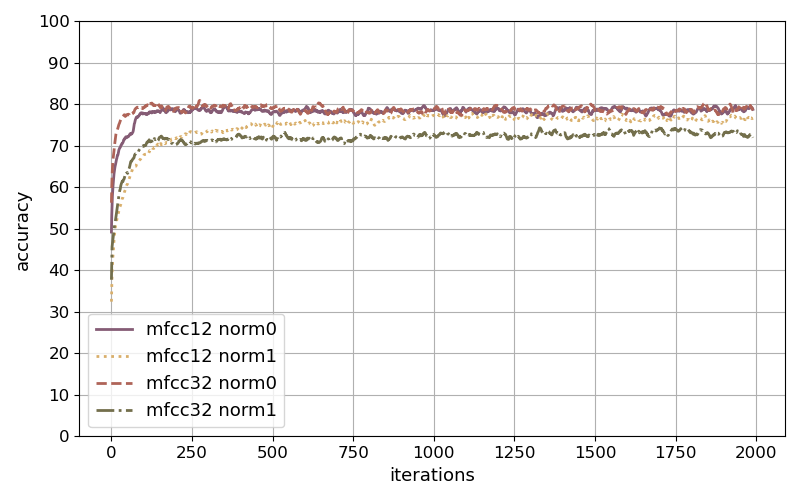
\includegraphics[width=0.48\textwidth]{../5_exp/figs/exp_fs_cepstral_acc_conv-trad.png}}
    \subfloat[conv-fstride]{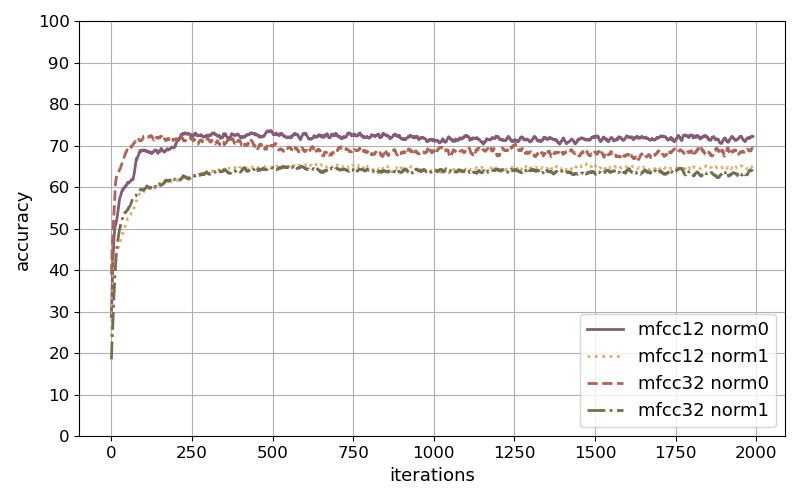
\includegraphics[width=0.48\textwidth]{../5_exp/figs/exp_fs_cepstral_acc_conv-fstride.png}}
  \end{figure}
\end{frame}

\begin{frame}
  \frametitle{Experiment: Feature Selection Cepstral Coeff.}
  \begin{figure}[!ht]
    \centering
    \subfloat[conv-jim]{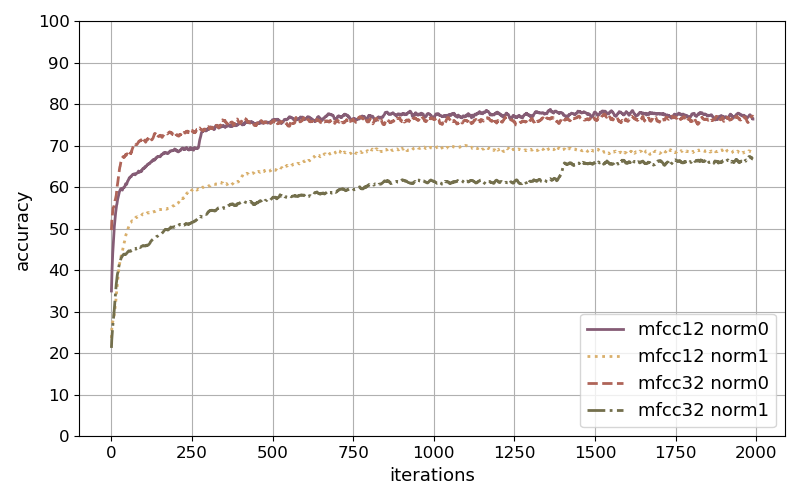
\includegraphics[width=0.75\textwidth]{../5_exp/figs/exp_fs_cepstral_acc_conv-jim.png}}
  \end{figure}
\end{frame}

\begin{frame}
  \frametitle{Experiment: Feature Selection Cepstral Coeff.}
  \begin{table}[ht!]
\scriptsize
\begin{center}
\begin{tabular}{ M{1.8cm}  M{1.5cm}  M{1cm}  M{2.2cm}  M{2.2cm} }
\toprule
\multirow{2}{1.8cm}{\centering\textbf{Model Name}} & \multirow{2}{1.5cm}{\centering\textbf{\# MFCC Coeffs.}} & \multirow{2}{*}{\centering\textbf{Norm.}} & \multicolumn{2}{c}{\textbf{Accuracy [\%]}}\\
&  &  & Test set & My dataset \\
\midrule
conv-trad & 12 & 0 & $80.57 \pm 0.34$ & $75.20 \pm 6.40$ \\
conv-trad & 12 & 1 & $76.17 \pm 1.02$ & $85.60 \pm 4.80$ \\
conv-trad & 32 & 0 & $79.77 \pm 1.56$ & $72.80 \pm 4.66$ \\
conv-trad & 32 & 1 & $74.63 \pm 1.13$ & $78.40 \pm 3.20$ \\
\midrule
conv-fstride & 12 & 0 & $72.03 \pm 1.94$ & $78.40 \pm 1.96$ \\
conv-fstride & 12 & 1 & $64.53 \pm 1.32$ & $72.00 \pm 2.53$ \\
conv-fstride & 32 & 0 & $70.73 \pm 1.42$ & $72.00 \pm 5.66$ \\
conv-fstride & 32 & 1 & $62.63 \pm 1.79$ & $69.60 \pm 4.80$ \\
\midrule
conv-jim & 12 & 0 & $78.70 \pm 1.38$ & $76.00 \pm 8.76$ \\
conv-jim & 12 & 1 & $72.90 \pm 1.85$ & $64.00 \pm 8.39$ \\
conv-jim & 32 & 0 & $76.40 \pm 3.22$ & $77.60 \pm 5.43$ \\
conv-jim & 32 & 1 & $65.83 \pm 1.29$ & $65.60 \pm 5.43$ \\
\bottomrule
\end{tabular}
\end{center}
\end{table}
\end{frame}

\begin{frame}
  \frametitle{Experiment: MFCC Enhancements}
  \begin{itemize}
    \item run on conv-jim model with frame-based normalization and 12 MFCC
    \item evaluation of
    \begin{itemize}
     \item different enhancements (c: cepstral, d: delta, dd: double delta, e: energy vector(s))
    \end{itemize}
    \item validation accuracy of best enhancement combination:
  \end{itemize}
  \vspace{-0.5cm}
  \begin{figure}[!ht]
    \centering
    \subfloat{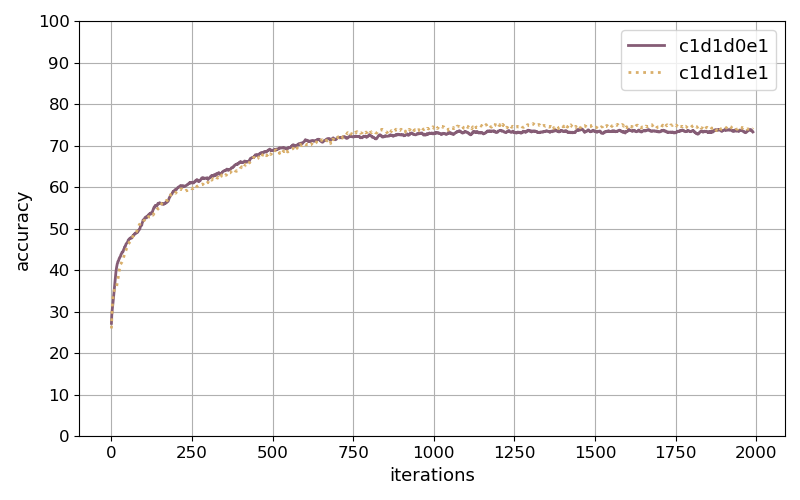
\includegraphics[width=0.48\textwidth]{../5_exp/figs/exp_fs_mfcc_acc_conv-jim.png}}
  \end{figure}
\end{frame}

\begin{frame}
  \frametitle{Experiment: MFCC Enhancements}
  \begin{table}[ht!]
\scriptsize
\begin{center}
\begin{tabular}{ M{0.75cm}  M{0.75cm}  M{0.75cm}  M{0.75cm}  M{2.5cm}  M{2.5cm} }
\toprule
\multicolumn{4}{c}{\textbf{Feature Selection}} & \multicolumn{2}{c}{\textbf{Accuracy [\%]}}\\
c & d & dd & e & Test set & My dataset\\
\midrule
0 & 0 & 1 & 0 & $37.40 \pm 2.17$ & $34.40 \pm 11.20$ \\
0 & 0 & 1 & 1 & $46.63 \pm 2.87$ & $36.80 \pm 7.76$ \\
0 & 1 & 0 & 0 & $58.57 \pm 2.06$ & $64.80 \pm 4.66$ \\
0 & 1 & 0 & 1 & $62.00 \pm 1.82$ & $75.20 \pm 11.14$ \\
0 & 1 & 1 & 0 & $59.03 \pm 1.77$ & $56.00 \pm 9.47$ \\
0 & 1 & 1 & 1 & $61.60 \pm 2.28$ & $62.40 \pm 6.97$ \\
1 & 0 & 0 & 0 & $72.00 \pm 1.46$ & $85.60 \pm 1.96$ \\
1 & 0 & 0 & 1 & $72.83 \pm 1.22$ & $80.00 \pm 4.38$ \\
1 & 0 & 1 & 0 & $70.63 \pm 2.13$ & $84.00 \pm 8.76$ \\
1 & 0 & 1 & 1 & $72.36 \pm 2.27$ & $80.00 \pm 4.38$ \\
1 & 1 & 0 & 0 & $72.80 \pm 2.90$ & $88.80 \pm 6.88$ \\
1 & 1 & 0 & 1 & $75.30 \pm 1.38$ & $92.00 \pm 2.53$ \\
1 & 1 & 1 & 0 & $73.43 \pm 2.05$ & $84.80 \pm 5.88$ \\
1 & 1 & 1 & 1 & $73.73 \pm 1.66$ & $83.20 \pm 6.88$ \\
\bottomrule
\end{tabular}
\end{center}
\end{table}
\end{frame}

\begin{frame}
  \frametitle{Experiment: Adversarial Label Train}
  \begin{itemize}
    \item run on conv-jim model with frame-based normalization and 12 MFCC
    \item evaluation of
    \begin{itemize}
     \item adversarial label train with different training epochs
     \item usage of either D or G filter weights
    \end{itemize}
    \item validation accuracy:
    \vspace{-0.5cm}
    \begin{figure}[!ht]
    \centering
    \subfloat{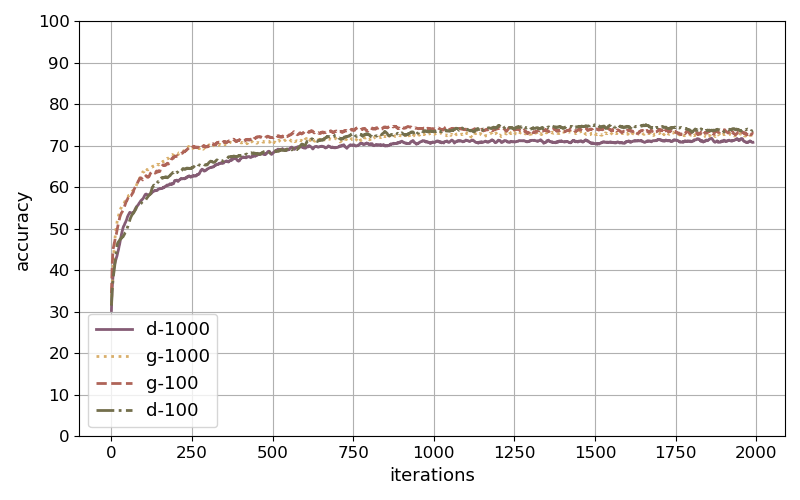
\includegraphics[width=0.48\textwidth]{../5_exp/figs/exp_adv_label_acc_conv-jim.png}}
    \end{figure}
  \end{itemize}
\end{frame}

\begin{frame}
  \frametitle{Experiment: Adversarial Label Train}
  \centering \vfill
  \begin{table}[ht!]
\scriptsize
\begin{center}
\begin{tabular}{ M{2cm}  M{2cm}  M{2.5cm}  M{2.5cm} }
\toprule
\multicolumn{2}{c}{\textbf{Adversarial}} & \multicolumn{2}{c}{\textbf{Accuracy [\%]}}\\
Epochs & Model & Test set & My dataset\\
\midrule
100 & G & $75.80 \pm 2.17$ & $85.60 \pm 4.08$ \\
100 & D & $73.57 \pm 1.59$ & $83.20 \pm 6.40$ \\
1000 & G & $74.83 \pm 2.15$ & $85.60 \pm 4.08$ \\
1000 & D & $73.36 \pm 0.86$ & $84.00 \pm 5.06$ \\
\bottomrule
\label{tab:exp_adv_label_l12}
\end{tabular}
\end{center}
\end{table}
\end{frame}

\begin{frame}
  \frametitle{Experiment: Wavenet}
  \begin{itemize}
    \item unfortunately poor classification results:
  \end{itemize}
  \vspace{-0.5cm}
  \begin{figure}[!ht]
    \centering
    \subfloat[validation accuracy]{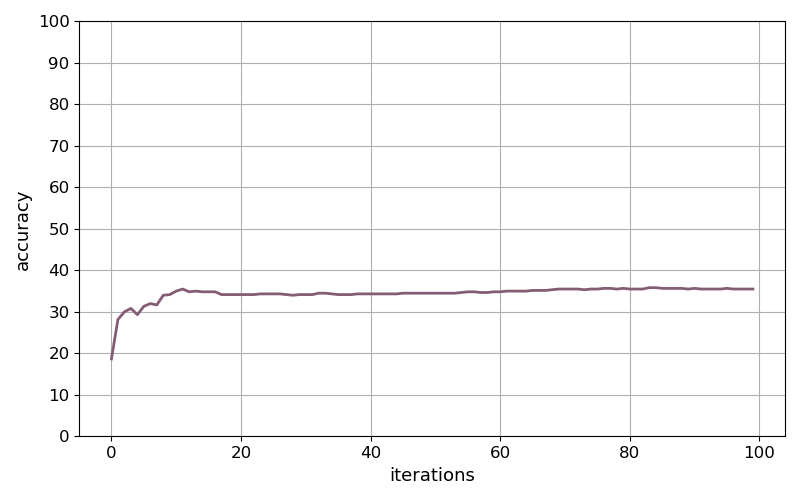
\includegraphics[width=0.45\textwidth]{../5_exp/figs/exp_wavenet_acc.png}}
    \subfloat[test confusion matrix]{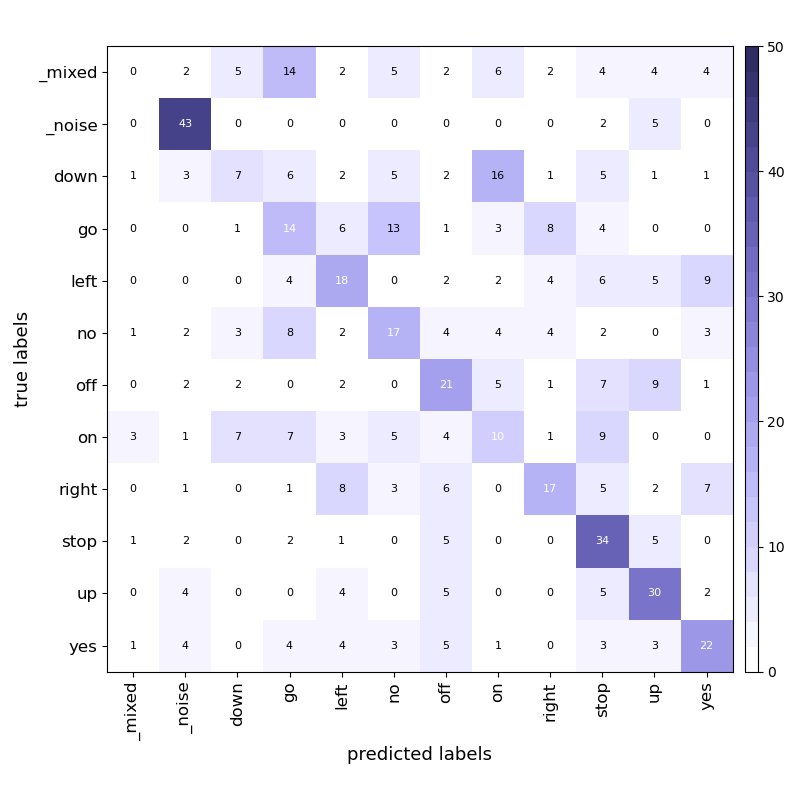
\includegraphics[width=0.45\textwidth]{../5_exp/figs/exp_wavenet_confusion_test.png}}
  \end{figure}
\end{frame}

\begin{frame}
  \frametitle{Experiment: Final}
  \begin{itemize}
    \item run on all CNN models the whole dataset
    \item evaluation of
    \begin{itemize}
     \item frame-based normalization
     \item adversarial label train
    \end{itemize}
    \item validation accuracy:
    \vspace{-0.5cm}
  \begin{figure}[!ht]
    \centering
    \subfloat[Norm.: 0]{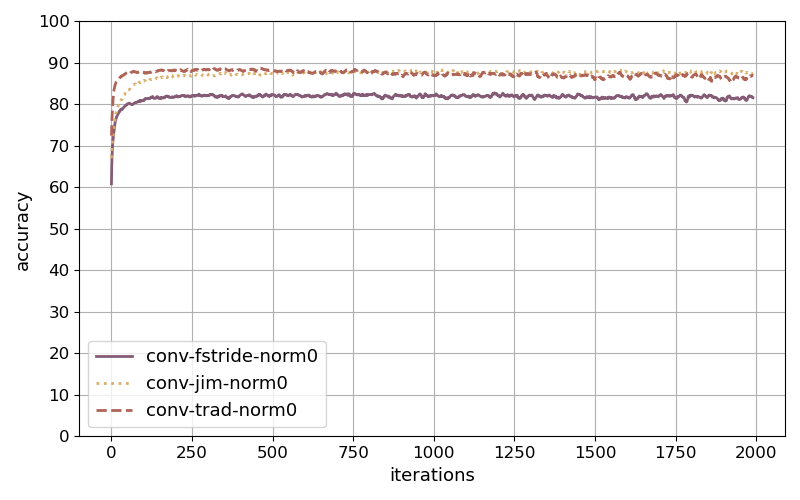
\includegraphics[width=0.48\textwidth]{../5_exp/figs/exp_final_acc_norm0.png}}
    \subfloat[Norm.: 1]{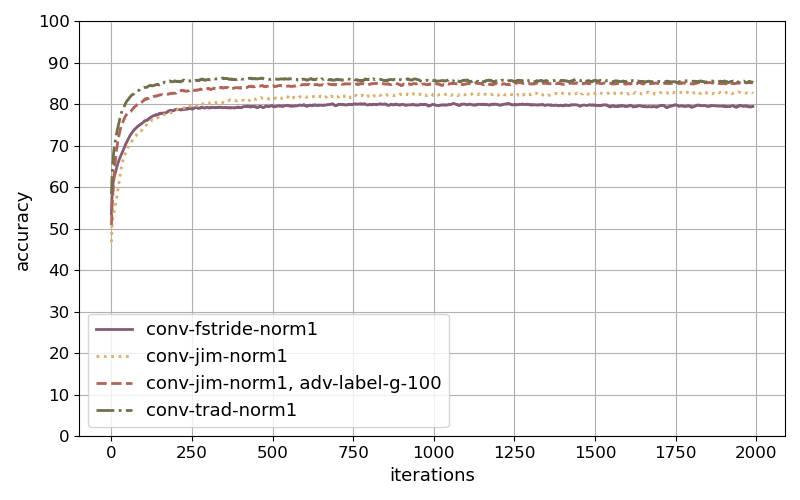
\includegraphics[width=0.48\textwidth]{../5_exp/figs/exp_final_acc_norm1.png}}
  \end{figure}
  \end{itemize}
\end{frame}

\begin{frame}
  \frametitle{Experiment: Final}
  \centering \vfill
  \begin{table}[ht!]
\scriptsize
\begin{center}
\begin{tabular}{ M{2cm}  M{1cm}  M{2cm}  M{1.75cm}  M{1.75cm} }
\toprule
\multirow{2}{*}{\centering\textbf{Model Name}} & \multirow{2}{*}{\centering\textbf{Norm.}} & \multirow{2}{*}{\centering\textbf{Pre-Train}} & \multicolumn{2}{c}{\textbf{Accuracy [\%]}}\\
& & & Test set & My dataset\\
\midrule
conv-trad & 0 & - & $84.52$ & $92.00$ \\
conv-fstride & 0 & - & $79.76$ & $80.00$ \\
conv-jim & 0 & - & $87.14$ & $88.00$ \\
\midrule
conv-trad & 1 & - & $83.79$ & $88.00$ \\
conv-fstride & 1 & - & $78.71$ & $92.00$ \\
conv-jim & 1 & - & $82.36$ & $88.00$ \\
\midrule
conv-jim & 1 & adv-label-100 & $84.62$ & $92.00$ \\
\bottomrule
\label{tab:exp_final_l12}
\end{tabular}
\end{center}
\end{table}
\end{frame}

\begin{frame}
  \frametitle{Experiment: Final}
  \begin{itemize}
      \item chosen model: conv-jim, frame-based normalized, adv-label-train
      \item confusion matrix on test set:
  \end{itemize}
  \begin{figure}[!ht] 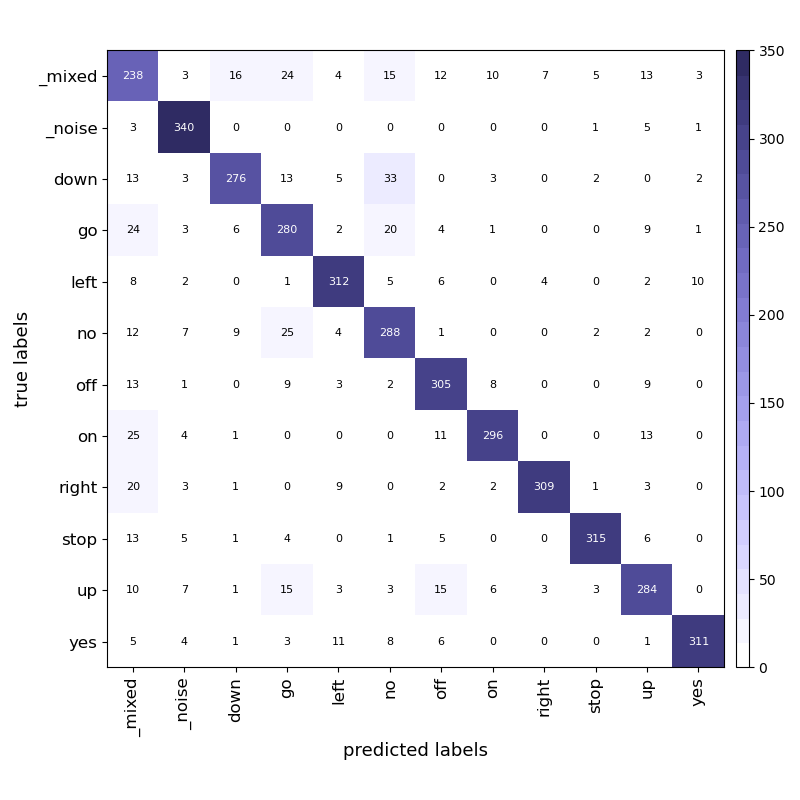
\includegraphics[width=0.45\textwidth]{../5_exp/figs/exp_final_confusion.png} \end{figure}
\end{frame}

% game (optional)

% conclusion
% --
% conclusion

\section{Conclusion}
\sectionheader{Conclusion}
\begin{frame}
  \frametitle{Conclusion}
  \begin{itemize}
    \item Conclusions on Signal length:
    \begin{itemize}
      \item reducing the speech signal to \SI{500}{\milli\second} was required to ensure a fast playing experience
      \item the energy onset detection method on the first cepstral coeff. was an efficient and accurate choice to detect the start of the keywords of the dataset examples.
      \item disadvantage: high possibility that not each phoneme of long words are captured.
    \end{itemize}
    \begin{figure} 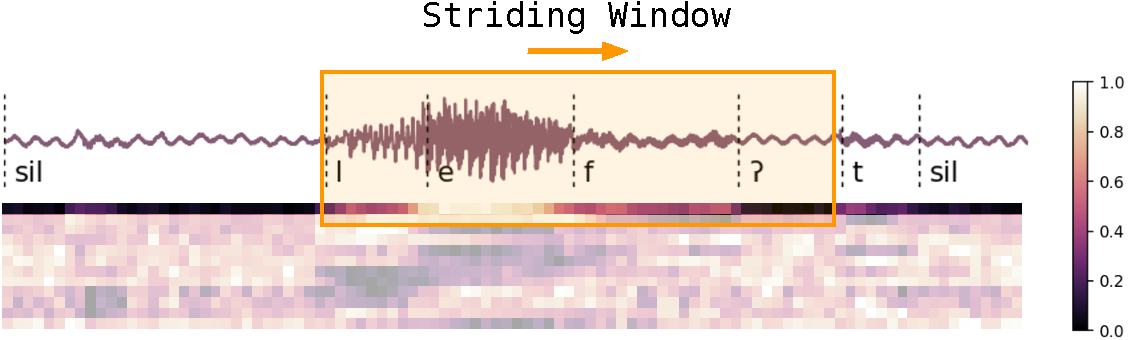
\includegraphics[width=0.6\textwidth]{../3_signal/figs/signal_onset_window.pdf} \end{figure}
  \end{itemize}
\end{frame}

\begin{frame}
  \frametitle{Conclusion}
  \begin{itemize}
    \item Conclusions based on the experiments of MFCC with CNNs:
    \begin{itemize}
      \item 32 MFCC coeff. are often worse than 12 MFCC coeff. for the tested models
      \item frame-based normalization decreases the classification accuracy, but improves noise invariance as for selected conv-jim models:
      \vspace{-0.5cm}
      \begin{figure}[!ht]
        \centering
        \subfloat[\#MFCC: 12, Norm.: 0]{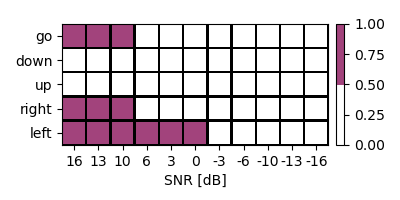
\includegraphics[width=0.3\textwidth]{../5_exp/figs/exp_fs_cepstral_tb_noise_conv-jim_mfcc12_norm0.png}}
        \qquad
        \subfloat[\#MFCC: 12, Norm.: 1]{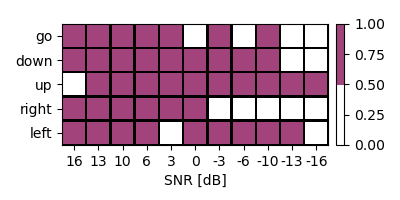
\includegraphics[width=0.3\textwidth]{../5_exp/figs/exp_fs_cepstral_tb_noise_conv-jim_mfcc12_norm1.png}}
      \end{figure}
      \item feature enhancements can improve the classification results, however, double delta features often worsens them.
    \end{itemize}
  \end{itemize}
\end{frame}

\begin{frame}
  \frametitle{Conclusion}
  \begin{itemize}
  \item Conclusions based on the adversarial label train:
    \begin{itemize}
      \item frame-based normalization is required
      \item slight improvement of the classification accuracy by applying the weights of the Generator model
      \item focusing of individual labels to train a specific amount of conv. filters is often better than training on the whole label set
    \end{itemize}
  \end{itemize}
\end{frame}


\end{document}